% Chapter nc_delta: Ramanujan's Delta in Thorin form (Volume II).
% Assembled from the salvage of four unrefereed notes of N. G. Polson (November 2026): "Ramanujan, the Tau Function and the Thorin Condition", "The Critical Region for the Tau Function", "Working the Open Problems" and "Working the Path: the de Bruijn Newman Flow for Delta in Thorin Form", following the Merge proposal sections and the MAJOR fixes of the referee reports misc/research/directions/opus/TAU1.md to TAU4.md.
% The flow material (Thorin flow, Laguerre form, Polya approximant, velocity table, gap remarks) is in ch/ch16.tex, Section sec:ch16:flowthorin.
% Numbers: only values that a report gives as checked or recomputed. Left out for lack of recomputed values: the flow columns of the power hierarchy table, the Monte Carlo table of hitting times, the prime sum table at level 13/2, and the truncation counts for K=3 and K=5.

This chapter carries the level $\alpha$ dictionary of the preceding chapter on Iwaniec's approach (Theorem~\ref{iw:thm:dictionary}) to Ramanujan's discriminant form $\Delta$, whose $L$ function $L(s,\Delta)=\sum\tau(n)n^{-s}$ has the same shape as $\zeta$ with every ingredient explicit: the kernel is a product, its log concavity is a two line computation, and Deligne's bound makes the Euler product positive in the sense of the sine squared lemma. It is assembled from unrefereed notes of Polson (November 2026) after a referee's reading, and only what survived that reading is kept. What is new relative to the book is Delta as an admissible $L$ function with the corrected L\'evy density, the Deligne compound Poisson remark, the Delta tables, a positivity argument by pairing zeros, the sphere identity for the kernel of $\Delta$, the Tur\'an table, a truncation test, and Ramanujan's lost notebook formula as a density. The de Bruijn Newman flow for $\Delta$ in Thorin form, is in Section~\ref{sec:ch16:flowthorin}, next to the flow of Section~\ref{sec:ch16:dbn}.

Every result carries one of the status words proved, computed, conditional, heuristic or open. The unrefereed zero free half plane of \cite{OAI26a} is never used as a theorem. No priority is claimed for anything below, and the identities that are classical (Jacobi's identity, the Hadamard product, Deligne's theorem) are credited as such. The answer to the question whether any of this is a path to the Riemann hypothesis for $\Delta$ is no (Section~\ref{dl:sec:path}).

\section{Setting and the dictionary for \texorpdfstring{$\Delta$}{Delta}}\label{dl:sec:setting}

Write $\Lambda(s)=(2\pi)^{-s}\Gamma(s)L(s,\Delta)=\int_0^\infty w^{s-1}\Delta(iw)\,dw$, entire, with $\Lambda(s)=\Lambda(12-s)$, real on $\mathbb R$, and positive on $\mathbb R$ because $\Delta(iw)=e^{-2\pi w}\prod_{n\ge1}(1-e^{-2\pi nw})^{24}>0$. Its zeros $\rho=\beta+i\gamma$ are the nontrivial zeros of $L(s,\Delta)$ and lie in $\frac{11}2<\beta<\frac{13}2$ (nonvanishing of $L(s,\Delta)$ on the edges of the strip). Put $\Theta_\Delta=\sup_\rho\beta$ and $\Xi_\Delta(t)=\Lambda(6+it)$, real and even; $\mathrm{RH}_\Delta$ is $\Theta_\Delta=6$. By Dobner's theorem \cite{Dobner21} and de Bruijn \cite{deBruijn} the de Bruijn Newman constant of $\Delta$ satisfies $0\le\Lambda_\Delta\le\frac18$ (Section~\ref{sec:ch16:dbn}). The kernel is $\Phi_\Delta(u)=e^{6u}\Delta(ie^u)=K_\Delta(u)$ of Section~\ref{sec:ch16:delta}, which is positive and even, and $V_\alpha$ is the variable with density $e^{(\alpha-6)u}\Phi_\Delta(u)/\Lambda(\alpha)$, so that $\mathbb E\,e^{itV_\alpha}=\Lambda(\alpha+it)/\Lambda(\alpha)$. The conditioned Gamma form $2\pi e^{V_\alpha}\overset d=(G_\alpha\,|\,M^*\le G_\alpha)$ and $L(\alpha,\Delta)=\mathbb P(M^*\le G_\alpha)$, with $M^*$ the maximum of $24$ independent copies of $\sup_nE_n/n$ as in Theorem~\ref{dl:thm:sphere}, are Corollary~\ref{cor:maxexp:forms} with $s=\alpha-\frac{11}2$: that corollary normalises $L(s,\Delta)$ to the line $\re s=\frac12$, and its $M^*$ is our $M^*/(2\pi)$; the Dirichlet series of $L(s,\Delta)$ does not converge absolutely in the critical strip, and the second identity holds there for real $\alpha$ regardless. Figure~\ref{dl:fig:phi} shows $\Phi_\Delta$ and $(\log\Phi_\Delta)''$.

\begin{figure}[htbp]
\centering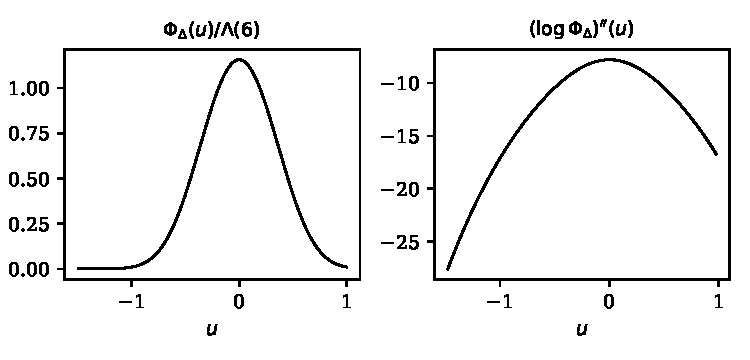
\includegraphics[width=\textwidth]{fig/nc_delta_phi.pdf}
\caption{The density of $V_6$ (left) and $(\log\Phi_\Delta)''$ (right), computed. The second derivative has maximum $-7.78927$ at $u=0$, below $-2\pi$.}
\label{dl:fig:phi}
\end{figure}

\begin{proposition}[Delta is admissible]\label{dl:prop:admissible}
The centred function $\Lambda^\circ(s)=\Lambda(s+\frac{11}2)$ is entire of order one, real on $\mathbb R$, satisfies $\Lambda^\circ(1-s)=\Lambda^\circ(s)$, and has its zeros in the open strip $0<\re s<1$. The level $\alpha$ dictionary, Theorem~\ref{iw:thm:dictionary}, therefore holds for $\Lambda^\circ$ verbatim, and in the unshifted variable it reads as follows. Status: proved.
\end{proposition}

\begin{theorem}[level $\alpha$ dictionary for $\Delta$]\label{dl:thm:level}
Let $\alpha\ge6$ and put $a_\rho=\alpha-\beta_\rho$. The following are equivalent: (a) $\Lambda$ has no zero with $\beta>\alpha$; (b) $\varphi_\alpha(s)=\Lambda(\alpha)/\Lambda(\alpha+\sqrt s)$ is the Laplace transform of a generalised gamma convolution; (c) $\re(\Lambda'/\Lambda)(s)>0$ for $\re s>\alpha$. When they hold the drift vanishes and the Thorin measure is $U_\alpha(dx)=\tilde u_\alpha(r)\,dr$ in the variable $r=\sqrt x$ on the part off the atoms, with
\[
\tilde u_\alpha(r)=\frac1\pi\re\frac{\Lambda'}\Lambda(\alpha+ir)=\frac1\pi\sum_\rho\frac{a_\rho}{a_\rho^2+(r-\gamma_\rho)^2}\qquad(\text{sum over all zeros}).
\]
For $\alpha>\Theta_\Delta$ the Thorin measure is absolutely continuous, and under $\mathrm{RH}_\Delta$ all heights equal $\alpha-6$. At $\alpha=\Theta_\Delta$ each zero with $\beta_\rho=\alpha$ gives an atom at $\gamma_\rho^2$ instead. Status: proved.
\end{theorem}

\begin{proof}
Proposition~\ref{dl:prop:admissible} and Theorem~\ref{iw:thm:dictionary} with the level $\alpha-\frac{11}2\ge\frac12$; the density is \eqref{iw:eq:thorindensity} in the variable $r$.
\end{proof}

\begin{corollary}\label{dl:cor:rh}
The following are equivalent: $\mathrm{RH}_\Delta$; $\Lambda(6)/\Lambda(6+\sqrt s)$ is a GGC transform; $\re(\Lambda'/\Lambda)(s)\ge0$ for $\re s>6$ (the Lagarias Hinkkanen criterion \cite{Lagarias} for $\Delta$). Under $\mathrm{RH}_\Delta$ the Thorin measure at level $6$ is $\sum_{\gamma>0}\delta_{\gamma^2}$, and $\tilde u_\alpha$ for $\alpha>6$ is the Poisson integral of $\sum_\rho\delta_{\gamma_\rho}$ at height $\alpha-6$. Unconditionally $\varphi_\alpha$ is a GGC transform for every $\alpha\ge\frac{13}2$. For $\xi$ the statements are Theorem~\ref{thm:poisson} and Corollary~\ref{iw:cor:qrh}. Status: proved.
\end{corollary}

The descent from a higher level to a lower one is the Cauchy semigroup $\tilde u_\alpha=P_{\alpha-\alpha'}*\tilde u_{\alpha'}$ of Theorem~\ref{iw:thm:semigroup}, for $\alpha>\alpha'\ge\Theta_\Delta$. It is legitimate exactly as long as the lower level stays at or above $\Theta_\Delta$; below it $\re\Lambda'/\Lambda$ has poles and the formal deconvolution produces a signed object.

\begin{remark}[the Thorin measure as an argument]\label{dl:rem:arg}
As in Proposition~\ref{prop:dbeta:arg} for $\chi_4$, for $\alpha>\Theta_\Delta$,
\[U_\alpha((0,R^2])=\int_0^R\tilde u_\alpha(r)\,dr=\frac1\pi\arg\Lambda(\alpha+iR),\]
with the argument continuous from $\Lambda(\alpha)>0$, and Stirling's formula gives
\[U_\alpha((0,R^2])=\frac R\pi\log\frac R{2\pi e}+\frac{2\alpha-1}4+S_\alpha(R)+O(R^{-1}),\qquad S_\alpha(R)=\frac1\pi\arg L(\alpha+iR,\Delta),\]
with $S_\alpha$ bounded for $\alpha>\frac{13}2$ (proved). So at every level the Thorin measure counts the zeros, each spread over a Cauchy window of width $\alpha-\beta_\rho$, and $\alpha\ge\Theta_\Delta$ exactly when $r\mapsto\arg\Lambda(\alpha'+ir)$ is nondecreasing for every $\alpha'>\alpha$. Under $\mathrm{RH}_\Delta$ the limit $\alpha\downarrow6$ is the Riemann von Mangoldt formula. Table~\ref{dl:tab:arg} gives the decomposition (computed, $110$ digits; for $\alpha=7$ the last column agrees with the Euler product over the primes below $10^5$ to $4\times10^{-4}$). This remark is from an unrefereed note of Polson (November 2026), with the table recomputed.
\end{remark}

\begin{table}[htbp]
\centering\small
\begin{tabular}{rrrrrr}
\toprule
$\alpha$ & $R$ & $N^+(R)$ & $U_\alpha((0,R^2])$ & main term & $S_\alpha(R)$\\
\midrule
$6.05$ & $20$ & $4$ & $3.9743$ & $3.5385$ & $0.4358$\\
$6.05$ & $40$ & $13$ & $13.0950$ & $13.4885$ & $-0.3935$\\
$6.05$ & $100$ & $59$ & $59.0301$ & $58.9808$ & $0.0493$\\
$6.5$ & $20$ & $4$ & $3.8944$ & $3.7232$ & $0.1712$\\
$6.5$ & $40$ & $13$ & $13.6030$ & $13.6929$ & $-0.0899$\\
$6.5$ & $100$ & $59$ & $59.2402$ & $59.1976$ & $0.0426$\\
$7$ & $20$ & $4$ & $4.0090$ & $3.9250$ & $0.0840$\\
$7$ & $40$ & $13$ & $13.8943$ & $13.9182$ & $-0.0239$\\
$7$ & $100$ & $59$ & $59.4627$ & $59.4376$ & $0.0251$\\
\bottomrule
\end{tabular}
\caption{The Thorin distribution function of $\Delta$ against the zero count and the archimedean main term $\frac1\pi(\arg\Gamma(\alpha+iR)-R\log2\pi)$, computed from $\arg\Lambda$.}\label{dl:tab:arg}
\end{table}

Strong log concavity: $-(\log K_\Delta)''(u)>2\pi e^{|u|}$ (Section~\ref{sec:ch16:dbn}), and the tilt $e^{(\alpha-6)u}$ does not change the second derivative. By the Brascamp Lieb inequality every $V_\alpha$ therefore satisfies $\operatorname{Var}V_\alpha=(\log\Lambda)''(\alpha)\le\frac1{2\pi}$ (proved). Under $\mathrm{RH}_\Delta$, $\operatorname{Var}V_6=\sum_\rho\gamma_\rho^{-2}$ over all zeros, and numerically $\operatorname{Var}V_6=0.1123518$, below $\frac1{2\pi}=0.159$ (computed).

\section{The L\'evy density and the role of the square root}\label{dl:sec:levy}

\begin{theorem}[L\'evy density]\label{dl:thm:levy}
Let $\alpha>\Theta_\Delta$. The GGC of Theorem~\ref{dl:thm:level} has L\'evy density
\begin{equation}\label{dl:eq:levy}
\ell_\alpha(x)=\frac1x\int_0^\infty e^{-xr^2}\tilde u_\alpha(r)\,dr=\frac1{2x}\sum_\rho\re\Bigl[e^{x(\alpha-\rho)^2}\operatorname{erfc}\bigl((\alpha-\rho)\sqrt x\bigr)\Bigr]\ \ge0,
\end{equation}
the sum over all zeros, and with $\ell_\alpha(x)=\frac{x^{-3/2}}{2\sqrt\pi}\sum_\rho\re\int_0^\infty e^{-(\alpha-\rho)y-y^2/(4x)}dy$. Status: proved.
\end{theorem}

\begin{proof}
For a GGC with Thorin measure $U$ and no drift, $-\log\varphi(s)=\int\log(1+s/x)U(dx)$, and Frullani's integral $\log(1+s/x)=\int_0^\infty(1-e^{-sy})e^{-xy}\,dy/y$ gives the L\'evy density $y^{-1}\int e^{-xy}U(dx)$. With $U(dx)=\tilde u_\alpha(r)dr$, $x=r^2$, this is the first form, positive because $\tilde u_\alpha\ge0$. For the second, put $c=\alpha-\rho$, $\re c=a_\rho>0$. The sum over the symmetric zero set makes $\re\sum_\rho(c+ir)^{-1}$ even in $r$, so $\int_0^\infty$ is half of $\int_{\mathbb R}$, and $\frac1\pi\int_{\mathbb R}e^{-xr^2}(c+ir)^{-1}dr=\frac c\pi\int_{\mathbb R}\frac{e^{-xr^2}}{c^2+r^2}\,dr=e^{xc^2}\operatorname{erfc}(c\sqrt x)$, the Laplace transform of a Cauchy density. The third form uses $e^{-y\sqrt s}=\int_0^\infty e^{-sx}\frac{y}{2\sqrt\pi}x^{-3/2}e^{-y^2/(4x)}dx$. The terms of the series behave like $a_\rho/|c|^2$ because $e^{xc^2}\operatorname{erfc}(c\sqrt x)\sim(c\sqrt{\pi x})^{-1}$, so it converges for fixed $x>0$.
\end{proof}

\begin{remark}[the role of $\sqrt s$]\label{dl:rem:sqrt}
Without the square root, each conjugate pair $\{\rho,\bar\rho\}$ with $a_\rho>0$ contributes to $\log\Lambda(\alpha+z)/\Lambda(\alpha)$ the signed L\'evy density $2e^{-ay}\cos(\gamma y)/y$ in $\int_0^\infty(1-e^{-zy})(\cdot)\,dy$, by Frullani's integral with $\re c=a>0$. This oscillates with the ordinate. We make no claim about the sum over all pairs, which does not converge pointwise in $y$ (the terms do not decay); since $\Lambda(\alpha+z)$ vanishes at $z=\rho-\alpha\notin(-\infty,0]$, the reciprocal $\Lambda(\alpha)/\Lambda(\alpha+z)$ is never a GGC transform (proved). Subordination by the stable$(\frac12)$ subordinator replaces $e^{-zy}$ by a Gaussian average over $y$, and the Gaussian average of $e^{-ay}\cos\gamma y$ is $\re[e^{xc^2}\operatorname{erfc}(c\sqrt x)]$, which is positive for $a>0$.
\end{remark}

\begin{proposition}[Deligne and the compound Poisson law]\label{dl:prop:deligne}
Write $\tau(p)=2p^{11/2}\cos\theta_p$. For $\re w>1$,
\[
\frac{\zeta(w)^2}{L(w+\frac{11}2,\Delta)}=\exp\Bigl(\sum_p\sum_{k\ge1}\frac{4\sin^2(k\theta_p/2)}{k}\,p^{-kw}\Bigr).
\]
All coefficients $4\sin^2(k\theta_p/2)/k$ are nonnegative if and only if $|\tau(p)|\le2p^{11/2}$ for every prime $p$. Hence Ramanujan's conjecture (Deligne's theorem \cite{Deligne74}) is equivalent to the statement that for each $\sigma>1$, $t\mapsto\zeta(\sigma+it)^2L(\sigma+\frac{11}2,\Delta)/\bigl(\zeta(\sigma)^2L(\sigma+it+\frac{11}2,\Delta)\bigr)$ is the characteristic function of a compound Poisson law on $\{-k\log p\}$ with L\'evy measure $\sum_{p,k}\frac{4\sin^2(k\theta_p/2)}{k}p^{-k\sigma}\delta_{-k\log p}$. Status: proved.
\end{proposition}

\begin{proof}
Expand $\log L(s,\Delta)=\sum_p\sum_k\frac{2\cos k\theta_p}kp^{k(11/2-s)}$ and $2\log\zeta(w)=\sum_p\sum_k\frac2kp^{-kw}$, and use $2-2\cos k\theta=4\sin^2(k\theta/2)$. If $|\tau(p)|\le2p^{11/2}$ then $\theta_p$ is real and the coefficients are nonnegative. If $|\tau(p)|>2p^{11/2}$ then $\theta_p=i\eta$ or $\theta_p=\pi+i\eta$ with $\eta\ne0$, and the coefficient at $k=2$ is $\frac12(2-2\cosh2\eta)<0$.
\end{proof}

This is the only place where Deligne's bound enters. For $\zeta$ the Euler product L\'evy measure is positive for free, and the measure here is discrete, so the law is infinitely divisible but not a GGC; the archimedean factor and the square root produce the continuous Thorin density of Theorem~\ref{dl:thm:level}. For $\alpha>\frac{13}2$ the logarithmic derivative is an absolutely convergent prime sum, and
\begin{equation}\label{dl:eq:primes}
\tilde u_\alpha(r)=\frac1\pi\Bigl[\re\psi(\alpha+ir)-\log2\pi-\sum_p\sum_{k\ge1}2\cos(k\theta_p)\log p\;p^{-k(\alpha-11/2)}\cos(kr\log p)\Bigr],
\end{equation}
the Weil explicit formula for $\Delta$ at the Poisson kernel of height $\alpha-6$ (proved); the prime side converges absolutely exactly when $\alpha>\frac{13}2$, and conditionally at $\alpha=\frac{13}2$.

\subsection{Hecke relations and the sign of the prime density}\label{dl:sec:hecke}

The Euler part of the Thorin density is a signed sum, and the Hecke relations describe its signs exactly. This subsection is from an unrefereed note of Polson (November 2026). Let $f$ be a holomorphic Hecke eigenform of level one and weight $k$, with $L(s,f)=\sum\lambda_f(n)n^{-s}$ normalised so that the critical line is $\re s=\frac12$, and $\lambda_f(p)=2\cos\theta_p$ with $\theta_p\in[0,\pi]$ by Deligne's theorem \cite{Deligne74}. For $\Delta$, $\lambda_\Delta(n)=\tau(n)n^{-11/2}$, and the centred level $\beta>1$ used in this subsection is $\beta=\alpha-\frac{11}2$. For $t\in\mathbb R$ put
\begin{gather*}
S_{f,\beta}(t)=\sum_p\sum_{m\ge1}2\cos(m\theta_p)\log p\;p^{-m\beta}\bigl(1-\cos(mt\log p)\bigr),\\
S_{\zeta,\beta}(t)=\sum_p\sum_{m\ge1}\log p\;p^{-m\beta}\bigl(1-\cos(mt\log p)\bigr)\ge0,
\end{gather*}
the prime parts of $\re(L'/L)(\beta+it)-(L'/L)(\beta)$ for $L=L(s,f)$ and $L=\zeta$. For $\Delta$ the compensated density $\tau_\alpha$ of Proposition~\ref{dl:prop:minorigin}, defined in Section~\ref{dl:sec:minorigin}, is $\pi\tau_\alpha(t)=\re\psi(\alpha+it)-\psi(\alpha)+S_{\Delta,\beta}(t)$.

\begin{lemma}\label{dl:lem:neg}
Every eigenform $f$ has a prime $p_0$ with $\lambda_f(p_0)<0$. Status: proved.
\end{lemma}

\begin{proof}
If $\lambda_f(p)\ge0$ for all $p$, then $0\le\lambda_f(p)\le2$ gives $\lambda_f(p)\ge\lambda_f(p)^2/2$. The Rankin Selberg $L$ function $L(s,f\times f)=\zeta(s)L(s,\mathrm{sym}^2f)$ and the prime number theorem for it give $\sum_{p\le x}\lambda_f(p)^2\log p\sim x$, hence $\sum_{p\le x}\lambda_f(p)\log p\ge x/3$ for large $x$. This contradicts the prime number theorem for $L(s,f)$, which gives $o(x)$ \cite[Ch.~5]{IwaniecKowalski04}.
\end{proof}

\begin{theorem}[no eigenform is a GGC on the Euler side]\label{dl:thm:never}
For every eigenform $f$ of level one and every $\beta>1$, $S_{f,\beta}(t)<0$ on an interval of $t$. Hence the compensated reciprocal of $L(s,f)$ at level $\beta$, whose Thorin density would be $S_{f,\beta}/\pi$, is never a generalised gamma convolution, whereas $S_{\zeta,\beta}\ge0$. Status: proved.
\end{theorem}

\begin{proof}
Write $S_{f,\beta}=\sum_pS_p$ with $S_p(t)=\log p\sum_{m\ge1}2\cos(m\theta_p)x_p^m(1-\cos(mt\log p))$ and $x_p=p^{-\beta}<\frac12$. Take $p_0$ from Lemma~\ref{dl:lem:neg}, so $\cos\theta_{p_0}<0$. Given $\varepsilon>0$ choose $P$ with $\sum_{p>P}|S_p(t)|<\varepsilon$ for all $t$. The numbers $\log p$, $p\le P$, are linearly independent over $\mathbb Q$, so Kronecker's theorem gives arbitrarily large $t$ with $t\log p_0$ within $\delta$ of $\pi$ and $t\log p$ within $\delta$ of $0$ modulo $2\pi$ for the other $p\le P$. For such $t$ the primes $p\ne p_0$ contribute $O_P(\delta^2)$, and $S_{p_0}(t)$ is within $O(\delta)$ of
\[
4\log p_0\sum_{m\ \mathrm{odd}}\cos(m\theta_{p_0})x_{p_0}^m=4\log p_0\,\frac{x\cos\theta\,(1-x^2)}{|1-x^2e^{2i\theta}|^2}\Big|_{x=x_{p_0},\,\theta=\theta_{p_0}}<0 .
\]
Small $\varepsilon$ and $\delta$ give $S_{f,\beta}(t)<0$, and by continuity $S_{f,\beta}<0$ on an interval.
\end{proof}

This does not contradict Proposition~\ref{dl:prop:minorigin}: for $\Delta$ the archimedean part of $\pi\tau_\alpha$ dominates the signed Euler part, which is bounded by Proposition~\ref{dl:prop:hecke2sin}. It does show that the positivity of $\tau_\alpha$ never comes from the Euler product alone, and nothing in this subsection locates a zero.

\begin{proposition}[the Thorin form of Proposition~\ref{dl:prop:deligne}, both signs]\label{dl:prop:hecke2sin}
For every eigenform $f$, every $\beta>1$ and every $t$, $2S_{\zeta,\beta}(t)-S_{f,\beta}(t)\ge0$ and $2S_{\zeta,\beta}(t)+S_{f,\beta}(t)\ge0$, that is $|S_{f,\beta}|\le2S_{\zeta,\beta}$; the compensated reciprocals of $\zeta^2L(s,f)^{\mp1}$ are GGCs on the Euler side. Status: proved.
\end{proposition}

\begin{proof}
The weights of $2S_{\zeta,\beta}\mp S_{f,\beta}$ are $(2\mp2\cos m\theta_p)\log p\;p^{-m\beta}(1-\cos(mt\log p))$, and $2\mp2\cos m\theta_p$ equals $4\sin^2(m\theta_p/2)$ or $4\cos^2(m\theta_p/2)$.
\end{proof}

The sign $-$ is the weight $4\sin^2(m\theta_p/2)$ of Proposition~\ref{dl:prop:deligne} (exponent $k$ there), carried to a Thorin density by the sine squared lemma (equation~\eqref{eq:sin2}, in the chart $z\mapsto2z$); the sign $+$ is the product $\zeta^2L(s,f)$. Both need Deligne's bound, which makes $\theta_p$ real.

For a finitely supported real vector $c=(c_0,c_1,\dots)$ let $F_c$ be the Euler product $\prod_n L(s,\mathrm{sym}^nf)^{c_n}$, where $L(s,\mathrm{sym}^nf)=\prod_p\prod_{j=0}^n(1-e^{i(n-2j)\theta_p}p^{-s})^{-1}$ and $\mathrm{sym}^0$ gives $\zeta$, and put $\mathcal T_c(\varphi)=\sum_nc_nU_n(\cos\varphi)$ with $U_n$ the Chebyshev polynomial of the second kind. The local weights of $F_c$ at $p^m$ are $\mathcal T_c(m\theta_p)\log p$, and $S_{F_c,\beta}$ is defined as above with $2\cos(m\theta_p)$ replaced by $\mathcal T_c(m\theta_p)$. The Hecke cone is $K_{\rm Hecke}=\{c:\mathcal T_c\ge0\ \text{on}\ [0,\pi]\}$.

\begin{theorem}[the Hecke cone]\label{dl:thm:cone}
If $c\in K_{\rm Hecke}$ then $S_{F_c,\beta}\ge0$ for every eigenform $f$ and every $\beta>1$. By the Fej\'er Riesz theorem, $c\in K_{\rm Hecke}$ exactly when $\mathcal T_c(\varphi)=|Q(e^{i\varphi})|^2$ for a polynomial $Q$. In particular $L(s,\mathrm{sym}^nf\times\mathrm{sym}^nf)=\prod_{j=0}^nL(s,\mathrm{sym}^{2j}f)$, for which $\mathcal T_c=U_n^2$ by the Clebsch Gordan rule $U_aU_b=\sum_{j=0}^{\min(a,b)}U_{a+b-2j}$, always has $S_{F_c,\beta}\ge0$. Status: proved.
\end{theorem}

\begin{proof}
The weights of $S_{F_c,\beta}$ are $\mathcal T_c(m\theta_p)\log p\;p^{-m\beta}(1-\cos(mt\log p))\ge0$. Absolute convergence for $\beta>1$ needs only Deligne's bound.
\end{proof}

For $c\notin K_{\rm Hecke}$ the Kronecker argument of Theorem~\ref{dl:thm:never}, with Sato Tate equidistribution \cite{BLGHT11}, is expected to give negative values (not proved). The vector $(2,-1)$ is Proposition~\ref{dl:prop:hecke2sin}, and $(1,0,1)$ gives $\mathcal T_c=4\cos^2\varphi$, which is $L(s,f\times f)=\zeta(s)L(s,\mathrm{sym}^2f)$. The vector $(3,4,1)$ has nonnegative coefficients but is not in $K_{\rm Hecke}$: $\mathcal T_c=2+8\cos\varphi+4\cos^2\varphi$ equals $-2$ at $\varphi=\pi$. The vector $(5,4,1)$ is in it, with $\mathcal T_c=4(1+\cos\varphi)^2$, the Hecke analogue of the inequality $3+4\cos\varphi+\cos2\varphi=2(1+\cos\varphi)^2\ge0$ in de la Vall\'ee Poussin's proof that $\zeta(1+it)\ne0$.

\section{Tables for \texorpdfstring{$\Delta$}{Delta}}\label{dl:sec:tables}

The first ten zeros of $\Lambda(6+it)$ are $9.222379$, $13.90755$, $17.44278$, $19.65651$, $22.3361$, $25.27464$, $26.80439$, $28.83168$, $31.17821$, $32.77488$, and there are $27$ zeros with $0<t<60$ (computed, $60$ digit arithmetic, mpmath). Also $L(8,\Delta)=0.930707030$ from the Dirichlet series and from the Mellin integral, $\operatorname{Var}V_6=\Lambda''(6)/\Lambda(6)=0.1123518$ and $(\log\Phi_\Delta)''(0)=-7.78927$ (computed). Table~\ref{dl:tab:three} gives the Thorin density $\tilde u_7$ at level $7$ from the Mellin integral.

\begin{table}[htbp]
\centering\small
\begin{tabular}{rr}
\toprule
$r$ & $\tilde u_7(r)$ from the Mellin integral\\
\midrule
$0$ & $0.035637$\\
$5$ & $0.050093$\\
$9.2$ & $0.366345$\\
$15$ & $0.250536$\\
$30$ & $0.413036$\\
\bottomrule
\end{tabular}
\caption{The Thorin density of $\Lambda(7)/\Lambda(7+\sqrt s)$ in the variable $r=\sqrt x$, computed.}\label{dl:tab:three}
\end{table}

The prime formula \eqref{dl:eq:primes} with the $9592$ primes below $10^5$ gives $\tilde u_7(0)=0.0356376$, $\tilde u_7(60)=0.7421580$, $\tilde u_8(0)=0.07054393$, $\tilde u_8(60)=0.72204076$, against the Mellin values $0.0356367$, $0.7421590$, $0.07054393$, $0.72204076$: agreement to $10^{-6}$ at $\alpha=7$, where the truncation of the prime sum dominates, and to eight digits at $\alpha=8$. The Poisson sum over the $212$ zeros with $|\gamma|<150$ falls short at $r=0$ by $\frac{2(\alpha-6)}\pi\sum_{\gamma>150}\gamma^{-2}=0.00565(\alpha-6)$, the contribution of the zeros above $150$ (computed). This check is from an unrefereed note of Polson (November 2026).

Figure~\ref{dl:fig:descent} shows $\tilde u_\alpha$ for $\alpha=7,6.5,6.25,6.1$ directly from the Mellin integral. The Poisson bumps sharpen toward the zeros as $\alpha\downarrow6$, and the minimum over $0\le r\le35$ stays at $r=0$, between the pair $\pm9.2224$ (Table~\ref{dl:tab:min}). From the theorem, $\tilde u_\alpha(0)=\frac1\pi\sum_\rho a_\rho/(a_\rho^2+\gamma_\rho^2)$, so under $\mathrm{RH}_\Delta$, $\tilde u_\alpha(0)/(\alpha-6)$ increases to $\operatorname{Var}V_6/\pi=0.035763$ as $\alpha\downarrow6$. Unconditionally,
\[\tilde u_\alpha(0)=\frac1\pi\frac{\Lambda'}\Lambda(\alpha)\ge\frac{(\alpha-6)\operatorname{Var}V_6}\pi\,\frac{\Lambda(6)}{\Lambda(\alpha)}\qquad(\alpha>6),\]
since $\frac{\Lambda'}\Lambda(6+x)=\mathbb E[V_6\sinh xV_6]/\mathbb E\cosh xV_6$ and $v\sinh xv\ge xv^2$ (proved). The ratio of the bound to the true value is $0.99998$ at $\alpha=6.02$, $0.9869$ at $6.5$ and $0.811$ at $8$ (computed). This bound is from an unrefereed note of Polson (November 2026).

\begin{figure}[htbp]
\centering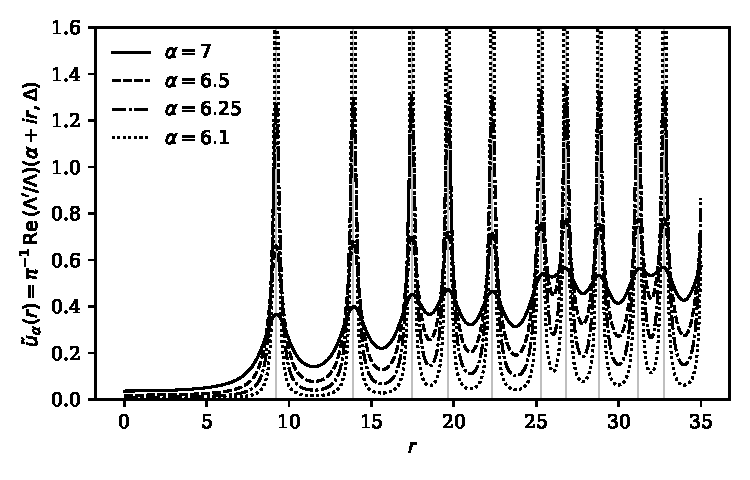
\includegraphics[width=\textwidth]{fig/nc_delta_descent.pdf}
\caption{Descent of the Thorin density toward the critical line, computed. Vertical lines are the zeros of $\Lambda(6+it)$: $9.2224$, $13.9075$, $17.4428$, $19.6565$, $22.3361$, $25.2746$, $26.8044$, $28.8317$, $31.1782$, $32.7749$.}
\label{dl:fig:descent}
\end{figure}

\begin{table}[htbp]
\centering\small
\begin{tabular}{rrr}
\toprule
$\alpha$ & $\min_{0\le r\le35}\tilde u_\alpha(r)$ & $\min/(\alpha-6)$\\
\midrule
$7$ & $0.035637$ & $0.035637$\\
$6.5$ & $0.017865$ & $0.035731$\\
$6.1$ & $0.003576$ & $0.035761$\\
$6.02$ & $0.000715$ & $0.035763$\\
\bottomrule
\end{tabular}
\caption{The minimum of the Thorin density as the level descends, computed; it is attained at $r=0$ and scales like $\alpha-6$, with ratio increasing to $0.035763$.}\label{dl:tab:min}
\end{table}

\subsection{Positivity on a window by pairing zeros}

\begin{proposition}\label{dl:prop:window}
Assume Keiper's computation \cite{NCKeiper96} that every zero of $\Lambda$ with $|\gamma|\le6397$ lies on $\re s=6$. Then $\tilde u_\alpha(r)>0$ for every $\alpha>6$ and every $|r|\le6396$, whatever the real parts of the zeros above $6397$. Status: proved, given the cited computation.
\end{proposition}

\begin{proof}
For $\alpha>\frac{13}2$ every $a_\rho>0$. Let $6<\alpha\le\frac{13}2$. Zeros on the line contribute positive Poisson terms of height $\alpha-6$. The zero set is invariant under $\rho\mapsto12-\bar\rho$, which keeps the ordinate and replaces $\beta$ by $12-\beta$; group each off line zero $\rho$ with this partner. With $a=\alpha-\beta$, $a'=\alpha-12+\beta$ and $d=r-\gamma$, the two Poisson terms sum to
\[
\frac a{a^2+d^2}+\frac{a'}{a'^2+d^2}=\frac{(a+a')(aa'+d^2)}{(a^2+d^2)(a'^2+d^2)},
\]
with $a+a'=2(\alpha-6)>0$ and $aa'=(\alpha-6)^2-(6-\beta)^2>-\frac14$. Every off line zero has $|\gamma|>6397$, so $|d|>1$ for $|r|\le6396$, and the sum is positive.
\end{proof}

This replaces a tempting but wrong argument that bounds the far zeros by $O(a_\rho/\gamma_\rho^2)$ with $|a_\rho|\le\frac12$ and compares with the local terms; that comparison fails for $\alpha-6<0.0035$ near $r=0$, where the local value is $0.0358(\alpha-6)$ and the far zeros could contribute about $1.3\times10^{-4}$ in absolute value.

\subsection{Tur\'an inequalities}

Under $\mathrm{RH}_\Delta$, $\Xi_\Delta(t)=\Lambda(6)\prod_{\gamma>0}(1-t^2/\gamma^2)$ is in the Laguerre P\'olya class. Write $\Xi_\Delta(t)/\Xi_\Delta(0)=\sum_k(-1)^km_{2k}t^{2k}/(2k)!$ with $m_{2k}=\mathbb E\,V_6^{2k}$. The Tur\'an inequalities, necessary for $\mathrm{RH}_\Delta$ (Csordas, Norfolk and Varga \cite{CNV86} proved the analogue for $\xi$), read
\begin{equation}\label{dl:eq:turan}
\frac{2k-1}{2k+1}\ \le\ \frac{m_{2k}^2}{m_{2k-2}m_{2k+2}}\ \le\ 1,\qquad k\ge1,
\end{equation}
the upper bound being Cauchy Schwarz for any law. Table~\ref{dl:tab:turan} gives the ratio from moments in $60$ digit arithmetic, recomputed by the referee for all rows: no violation for $k\le40$, with a margin that peaks at $0.0344$ near $k=3$ (at $k=4$ it is $0.0329$) and then falls, more slowly than $1/k$ in the range computed. These conditions test forty moments of a law whose relevant zeros are all of them; they are weak, and they are what a counterexample would have to evade (computed).

\begin{table}[htbp]
\centering\small
\begin{tabular}{rrrr}
\toprule
$k$ & $m_{2k}^2/(m_{2k-2}m_{2k+2})$ & $(2k-1)/(2k+1)$ & margin\\
\midrule
$1$ & $0.355858$ & $0.333333$ & $0.0225$\\
$2$ & $0.633635$ & $0.600000$ & $0.0336$\\
$3$ & $0.748672$ & $0.714286$ & $0.0344$\\
$5$ & $0.849221$ & $0.818182$ & $0.0310$\\
$10$ & $0.927877$ & $0.904762$ & $0.0231$\\
$20$ & $0.966573$ & $0.951220$ & $0.0154$\\
$40$ & $0.984790$ & $0.975309$ & $0.0095$\\
\bottomrule
\end{tabular}
\caption{Tur\'an inequalities for $\Xi_\Delta$, computed; $m_2=\operatorname{Var}V_6=0.112352$, $m_4=0.035472$.}\label{dl:tab:turan}
\end{table}

\subsection{The minimum at the origin and the compensated density}\label{dl:sec:minorigin}

For $\alpha>6$ write $b_\alpha=(\Lambda'/\Lambda)(\alpha)$ and $v_\alpha(\theta)=\re(\Lambda'/\Lambda)(\alpha+i\theta)$, so that $\tilde u_\alpha(r)=v_\alpha(r)/\pi$ in Theorem~\ref{dl:thm:level} and $b_\alpha=v_\alpha(0)$. Since $\Lambda(6+h)$ is the Laplace transform of the positive even kernel $\Phi_\Delta$, $\log\Lambda$ is strictly convex on the real line and even about $6$, so $b_\alpha>0$. Put
\[
\tau_\alpha(r)=\tilde u_\alpha(r)-\tilde u_\alpha(0)=\frac{v_\alpha(r)-b_\alpha}\pi .
\]
This is not the Thorin density of $\Lambda(\alpha)/\Lambda(\alpha+\sqrt s)$: that density is $\tilde u_\alpha$, and $\tau_\alpha$ is its excess over the value at the origin, that is the density of the compensated function $e^{\sqrt s\,b_\alpha}\Lambda(\alpha)/\Lambda(\alpha+\sqrt s)$. In the variable $r=\sqrt x$ the compensation is a constant density, because $\frac1\pi\int_0^\infty\log(1+w^2/r^2)\,dr=w$. The positivity of $\tau_\alpha$ is therefore the property that $\tilde u_\alpha$ has its minimum at the origin, the property that Proposition~\ref{bp:prop:valpha} and Theorem~\ref{thm:dbeta:minall} give for $\xi$, $\chi_4$ and $\chi_{12}$, and it is not implied by the dictionary. Positivity of $\tilde u_\alpha$ itself holds for $\alpha\ge\frac{13}2$ by Corollary~\ref{dl:cor:rh}, with no computation.

\begin{proposition}\label{dl:prop:minorigin}
(a) Whenever the representation of Theorem~\ref{dl:thm:level} holds at level $\alpha$, in particular for $\alpha\ge\frac{13}2$ and under $\mathrm{RH}_\Delta$, $\log\big(e^{\sqrt s\,b_\alpha}\Lambda(\alpha)/\Lambda(\alpha+\sqrt s)\big)=-\int_0^\infty\log(1+s/r^2)\,\tau_\alpha(r)\,dr$, so the compensated function is the Laplace transform of a generalised gamma convolution with no drift and Thorin density $\tau_\alpha$ exactly when $\tau_\alpha\ge0$. Status: proved.

(b) If $\tau_\alpha(r)>0$ for every $r\ne0$ and every $\alpha>6$, then $\mathrm{RH}_\Delta$ holds. Status: proved.

(c) $\mathrm{RH}_\Delta$ holds if and only if $\tau_\alpha(r)>0$ for every $r\ne0$ on every line $6<\alpha<\frac{13}2$, and no gap condition on the zeros is needed. Moreover $\tau_\alpha(r)>0$ for $0<|r|\le6397-\frac{1+\sqrt2}2$ when $6<\alpha\le12.4$, and for every $r\ne0$ when $6.7071\le\alpha\le12.4$, with no hypothesis on the zeros. Status: conditional on the constants of the column for $\Delta$ of Table~\ref{tab:dbeta:minall}, which are computed in floating point; certification in ball arithmetic is pending. The range $0<|r|\le6397-\frac{1+\sqrt2}2$ is also conditional on Keiper's computation \cite{NCKeiper96}, as in Proposition~\ref{dl:prop:window}.
\end{proposition}

\begin{proof}
(a) By Theorem~\ref{dl:thm:level}, $\log(\Lambda(\alpha+\sqrt s)/\Lambda(\alpha))=\int_0^\infty\log(1+s/r^2)\tilde u_\alpha(r)\,dr$; add $\sqrt s\,b_\alpha=\int_0^\infty\log(1+s/r^2)\tilde u_\alpha(0)\,dr$. (b) $\tau_\alpha>0$ gives $v_\alpha(\theta)>b_\alpha>0$, hence $\re(\Lambda'/\Lambda)(s)>0$ for $\re s>6$, and Corollary~\ref{dl:cor:rh} applies. (c) This is parts (ii$_\Delta$), (iii$_\Delta$) and (vi$_\Delta$) of Remark~\ref{bp:rem:deltacol}, that is Theorem~\ref{thm:dbeta:minall} transferred to $\Delta$; its proof uses of the zeros only the first ordinate and Keiper's height, through the comparison across vertical lines (Theorem~\ref{thm:dbeta:comp}, zero side) and the explicit lower bound of Corollary~\ref{cor:dbeta:lower}, which for $\Delta$ rests on Deligne's bound.
\end{proof}

The shorter route of Remark~\ref{rem:dbeta:nearest} needs a gap condition; Theorem~\ref{thm:dbeta:minall} and (c) do not. Nothing here shows that positivity of $\tau_\alpha$ is stronger than $\mathrm{RH}_\Delta$: by (c) its positivity on the lines $6<\alpha<\frac{13}2$ is equivalent to it, once the constants are certified; positivity for $\alpha>12.4$ is computed below, from a prime sum argument. For $\alpha=6$ the compensation is empty, since $b_6=0$, and $\tau_6=\tilde u_6$.

The book computed the property earlier only on windows (Table~\ref{dl:tab:min}: $\alpha=7$, $6.5$, $6.1$, $6.02$, $r\le35$, minimum at $r=0$). At $\alpha=7$, $b_7=0.1119559=\pi\cdot0.035637$, the value at $r=0$ of Table~\ref{dl:tab:three}. Beyond $\alpha=7$ a further computed check from the Hecke expansion at high precision is that $\pi\tau_9$ has minimum $0.002805$ on $[1,40]$, at $r=1$, and $\pi\tau_8$ has minimum $0.000534$ on $[0.5,40]$, at $r=0.5$; these are checks, not certificates. The compensated density, and the idea of a floating point argument for it from the prime sum at large $\alpha$, are those of an unrefereed note of Polson (November 2026); that note calls $\tau_\alpha$ the Thorin density of $1/\Lambda$, which the identification above corrects, and its prime sum argument is the one used next.

The prime sum argument of the same note gives $\tau_\alpha(r)\ge0$ for every $\alpha\ge8.25$, so that with part (iii$_\Delta$) of Remark~\ref{bp:rem:deltacol} $\tau_\alpha\ge0$ for every $\alpha\ge6.7071$ and $r\ne0$ (part (iv$_\Delta$) of that remark; computed in floating point, not certified).

The implication from $\mathrm{RH}_\Delta$ to positivity on the lines $6<\alpha<\frac{13}2$, which the same note leaves open, is Proposition~\ref{dl:prop:minorigin}(c). A scan on $0<r\le60$ with Taylor model enclosures gives $\tau_\alpha>0$ at the levels $\alpha=6.02$, $6.05$, $6.1$, $6.25$, $6.4$ and $6.5$ (computed), where the minimum over $0<r<2$ of $\pi\tau_\alpha(r)/((\alpha-6)r^2)$ is $1.198\cdot10^{-3}$ at the first three levels, $1.196\cdot10^{-3}$, $1.193\cdot10^{-3}$ and $1.189\cdot10^{-3}$ at the others, close to the limit $6\sum_{\gamma>0}\gamma^{-4}\approx1.20\cdot10^{-3}$ as $\alpha\downarrow6$. These are six computed levels and not a threshold over all levels.

Under GRH for $\Delta$ the positivity of $\tau_\alpha$ near the centre reduces to an inequality on all of $\mathbb R$. Let $Z(t)=\Lambda(6+it)$, real and even, with ordinates $\gamma$ (both signs), and put $g(t)=\sum_\gamma(t-\gamma)^{-2}=(Z'^2-ZZ'')/Z^2$ and $c=g(0)=\sum_\gamma\gamma^{-2}=\operatorname{Var}V_6=0.1123518$.

\begin{corollary}[strengthened Laguerre inequality]\label{dl:cor:laguerre}
Assume GRH for $\Delta$. Then $E=Z'^2-ZZ''-cZ^2\ge0$ on all of $\mathbb R$. Status: conditional on GRH for $\Delta$, and computed (one inequality between three special values, evaluated in floating point).
\end{corollary}

\begin{proof}
Under GRH $v_{6+a}(t)=\sum_\gamma a/(a^2+(t-\gamma)^2)$, and each term $1/(a^2+(t-\gamma)^2)$ of $v_{6+a}(t)/a$ decreases in $a$, so $g(t)\ge v_9(t)/3$ for every $t$ that is not an ordinate. By Remark~\ref{bp:rem:deltacol}, $v_9(t)\ge A(t)-S$ with $A(t)=-\log2\pi+\re\psi(9+it)$, which increases in $|t|$, and $S=-2\zeta'/\zeta(\frac72)$. Computed: $A(7)-S-3c=0.02327>0$, so $g(t)>c$ for $|t|\ge7$; the root of $A(t)-S=3c$ is $t=6.5940030$. For $|t|\le\sqrt3\gamma_1=15.97$, pairing $\gamma$ with $-\gamma$ gives $\frac1{(t-\gamma)^2}+\frac1{(t+\gamma)^2}-\frac2{\gamma^2}=\frac{2t^2(3\gamma^2-t^2)}{\gamma^2(\gamma^2-t^2)^2}\ge0$ for every $\gamma\ge\gamma_1$, so $g(t)\ge g(0)=c$. Hence $E=Z^2(g-c)\ge0$ off the ordinates, and $E=Z'^2\ge0$ at an ordinate.
\end{proof}

\subsection{The GHS inequality and the eta block}\label{dl:sec:ghs}

Put $K(h)=\log(\Lambda(6+h)/\Lambda(6))$, the cumulant generating function of $V_6$, an even function of $h$. GKS needs only evenness. For GHS one asks $K'''(h)<0$ for $h>0$, the inequality that Newman proved for $\xi$ \cite{Newman91}.

\begin{theorem}\label{dl:thm:ghs}
$K'''(h)<0$ for every $h\ge6.574$ (proved). On $(0,6.6]$ it is a computed fact: on a grid of step $0.02$ over $[0.02,6.6]$ the maximum of $K'''$ is $-4.794\times10^{-5}$, at $h=0.02$, and $K'''(1)=-0.0023251$. Near the origin $K'''(h)=\kappa_4h+O(h^3)$ with $\kappa_4=m_4-3m_2^2=-0.00240$ in the notation of Table~\ref{dl:tab:turan} (computed). Between grid points $K'''$ has not been bounded, so the range $(0,6.574)$ is a numerical check and not a proof.
\end{theorem}

\begin{proof}
For $s=6+h$, $K'''(h)=\psi''(s)-\sum_{n\ge2}\Lambda_\Delta(n)(\log n)^2n^{-s}$, where $-L'/L(s,\Delta)=\sum\Lambda_\Delta(n)n^{-s}$ and $|\Lambda_\Delta(n)|\le2n^{11/2}\Lambda(n)$ by Deligne \cite{Deligne74}. The prime sum is at most $B(h)=-2(\zeta'/\zeta)''(h+\frac12)$, finite for $h>\frac12$, and $\psi''(s)\le-1/s^2$. So $K'''<0$ as soon as $(6+h)^{-2}>B(h)$; the two sides cross at $h=6.57388$ ($B=0.00632501=(12.57388)^{-2}$) and $B$ decreases like $2^{-h}$, which gives the range $h\ge6.574$.
\end{proof}

A route to every $h\ge0$ is Newman's: the class of Ellis, Monroe and Newman \cite{EMN76} needs $F'$ convex on $[0,\infty)$ for $F=-\log\Phi_\Delta$, that is $F'''\ge0$. Computed values are $F''=7.78927$, $8.24716$, $17.07972$, $46.42681$ at $u=0$, $0.2$, $1$, $2$, increasing along a finer grid ($u=0.05,0.1,0.3,0.5$ give $7.81839$, $7.90534$, $8.79750$, $10.43300$), so GHS for $\Delta$ would follow from \cite{EMN76} once $F'''\ge0$ is proved, which is open.

The eta block. Let $\Phi_\eta(u)=e^{u/4}\eta(ie^u)$, positive and even by the modularity of $\eta$, so that $\Phi_\Delta=\Phi_\eta^{24}$. Let $U_1,\dots,U_{24}$ be independent with density $f=\Phi_\eta/\int\Phi_\eta$. Since $\sum_{i<j}(u_i-u_j)^2=23\sum u_i^2-2\sum_{i<j}u_iu_j$,
\[
\exp\Big(-\frac J2\sum_{i<j}(u_i-u_j)^2\Big)=\exp\Big(J\sum_{i<j}u_iu_j\Big)\prod_ie^{-23Ju_i^2/2},
\]
and as $J\to\infty$ the law of the block mean $\frac1{24}\sum U_i$ under this weight converges to the density proportional to $f^{24}$, that is the law of $V_6$. So $V_6$ is the strong coupling limit of a ferromagnetic block of $24$ spins, each with single spin measure $f(u)e^{-23Ju^2/2}du$.

\begin{proposition}\label{dl:prop:eta}
For every $\beta>0$ the measure $f(u)e^{-\beta u^2}du$ is not Lee Yang. Status: proved, given Dobner's theorem.
\end{proposition}

\begin{proof}
After the change of variable $s\mapsto2s$, which rescales $u$ and the time of the flow by a positive factor, its Fourier transform is the de Bruijn Newman deformation at negative time of the completed $L(2s,\chi_{12})$. $L(s,\chi_{12})$ is in the extended Selberg class, so its de Bruijn Newman constant is at least $0$ by Dobner \cite{Dobner21}, and every deformation at negative time has a nonreal zero.
\end{proof}

So the block cannot be realised with Lee Yang single spins for any coupling: the Gaussian damping of strong ferromagnetic coupling is a backward heat flow. GRH for $\chi_{12}$ (Lee Yang for $f$) and $\mathrm{RH}_\Delta$ (Lee Yang for $f^{24}$) are not known to imply one another. In weight $12$ and level $1$, an entire Dirichlet series with the factor $(2\pi)^{-s}\Gamma(s)$, bounded in vertical strips and with $\Lambda(s)=\Lambda(12-s)$, is a multiple of $L(s,\Delta)$ by Hecke's converse theorem \cite{Hecke36}, so the functional equation determines $\Delta$ and any obstruction must drop one of its hypotheses; the kernels $\Phi_\eta^k$ with $k\ne24$ have other weights and levels.

\subsection{A Putnam theorem for \texorpdfstring{$\Delta$}{Delta}}\label{dl:sec:putnam}

Write $\lambda(n)=\tau(n)n^{-11/2}$ and $L(s)=\sum\lambda(n)n^{-s}$, whose critical line is $\re s=\frac12$, so that $L(s)=L(s+\frac{11}2,\Delta)$ and $\Xi_\Delta(t)=0$ exactly when $L(\frac12+it)=0$. The periodisation argument of Putnam for $\zeta$ transfers to $\Delta$, as an unrefereed note of Polson (November 2026) observes; the proof below avoids pointwise values of the periodised function.

\begin{theorem}\label{dl:thm:putnam}
Let $d>0$ and $r=e^{2\pi/d}$. If no positive integer power of $r$ is an integer, or if $r^q=a$ for an integer $a$ (with $q\ge1$ minimal) and $H(a)=\sum_{j\ge0}\lambda(a^j)a^{-j/2}\ne0$, then $L(\frac12+idn)\ne0$ for some $n\ge1$. Status: conditional on the bound $S(y)=O(y^{1/3+\varepsilon})$ of the proof, for which no reference is yet verified.
\end{theorem}

\begin{proof}
Let $S(y)=\sum_{n\le y}\lambda(n)$. For a cusp form of level one $S(y)=O(y^{1/3+\varepsilon})$ for every $\varepsilon>0$ (the classical estimate for partial sums of cusp form coefficients), % UNCHECKED: reference for this bound; see misc/research/directions/opus/merge6_tauly_bib.txt
so $L(s)=s\int_0^\infty S(e^x)e^{-sx}\,dx$ for $\re s>\frac13$, with no pole term. Put $P=2\pi/d$, $g(x)=S(e^x)e^{-x/2}$ for $x\ge0$ and $g(x)=0$ for $x<0$. Then $|g(x)|\le Ce^{-cx}$ with $c=\frac16-\varepsilon>0$, and $L(\frac12+it)=(\frac12+it)\hat g(t)$. Suppose $L(\frac12+idn)=0$ for all $n\ge1$. Since $g$ is real, $\hat g(dn)=0$ for all $n\ne0$. The periodisation $D(x)=\sum_{k\in\mathbb Z}g(x+kP)$ converges absolutely and has Fourier coefficients $(d/2\pi)\hat g(dn)$, so $D$ is constant almost everywhere. Hence, for $0<\eta<\min(1,P)$,
\[
0=\frac1\eta\int_0^\eta D-\frac1\eta\int_{-\eta}^0D=\sum_{k\ge0}h_k(\eta),\qquad h_k(\eta)=\frac1\eta\Big(\int_{kP}^{kP+\eta}g-\int_{kP-\eta}^{kP}g\Big),
\]
since $g=0$ on $x<0$. The function $g$ is a step function times $e^{-x/2}$ with jumps only at $x=\log m$, so it has one sided limits at every point, and $g(x+)-g(x-)=J(x)$ with $J(x)=\lambda(m)m^{-1/2}$ if $e^x=m$ is an integer and $J(x)=0$ otherwise (at $x=0$, $J(0)=\lambda(1)=1$). So $h_k(\eta)\to J(kP)$ as $\eta\downarrow0$, and $|h_k(\eta)|\le2Ce^{-c(kP-1)}$ uniformly in $\eta$ and summably in $k$. By dominated convergence $\sum_{k\ge0}J(kP)=0$. Now $J(kP)\ne0$ requires $r^k=m$ to be an integer. If no positive power of $r$ is an integer only $k=0$ remains and the sum is $1$. Otherwise let $r^q=a$ with $q$ minimal and let $r^k$ be an integer; with $g_0=\gcd(k,q)$, $r^{g_0}$ is a product of integer powers of $r^k$ and $r^q$, hence rational, and some power of it is the integer $a$, so $r^{g_0}$ is an integer and $g_0=q$ by minimality. So $k=qj$, $m=a^j$, and the sum is $\sum_{j\ge0}\lambda(a^j)a^{-j/2}=H(a)$. In both cases the sum is not $0$, a contradiction.
\end{proof}

\begin{lemma}\label{dl:lem:putnamH}
$H(p^e)>0$ for every prime power $p^e$. Status: proved.
\end{lemma}

\begin{proof}
By Deligne \cite{Deligne74} $\lambda(p)=2\cos\theta_p$ with $\theta_p$ real, and $\sum_n\lambda(p^n)y^n=L_p(y)=((1-e^{i\theta_p}y)(1-e^{-i\theta_p}y))^{-1}$. Hence $H(p^e)=\frac1e\sum_{\omega^e=1}L_p(\omega p^{-1/2})$. For $|y|\le2^{-1/2}$ each factor $1/(1-u)$, $|u|<1$, has positive real part and argument at most $\frac\pi4$ in absolute value, so $L_p(y)$ has nonnegative real part. The term $\omega=1$ is real and positive, since the two factors are conjugate. $H$ is real, so $H(p^e)>0$.
\end{proof}

For $a$ with at least two distinct prime factors, $H(a)$ is a finite computation from the coefficients; for $a<3000$ it has no zero, and the least value of $|H(a)|$ over these $a$ is $0.857$, at $a=12$ (computed).

\begin{corollary}\label{dl:cor:putnam}
The law of $V_6$ has no independent uniform factor: it is not the law of $aU+W$ with $a>0$, $U$ uniform on $[-1,1]$ and $W$ independent of $U$, unless $r=e^{2a}$ has a power $r^q=a'$ that is an integer with at least two distinct prime factors and $H(a')=0$. Status: conditional, as Theorem~\ref{dl:thm:putnam}.
\end{corollary}

\begin{proof}
The characteristic function of $V_6$ is $\Xi_\Delta(t)/\Xi_\Delta(0)$; a factor $aU$ would contribute $\sin(at)/(at)$, so $\Xi_\Delta$ would vanish at $t=\pi n/a$ for every $n\ge1$, which is the case $d=\pi/a$ of Theorem~\ref{dl:thm:putnam}, excluded unless its hypothesis fails; by Lemma~\ref{dl:lem:putnamH} it fails only if $a'$ has at least two distinct prime factors.
\end{proof}

A uniform factor forces a homogeneous progression of zeros of $\Xi_\Delta$. For cosine power spins the progression $\pi(n+b)/a$ is inhomogeneous, and a theorem of the kind of Li and Radziwi\l\l\ for $L(s,\Delta)$ would be needed to exclude it; that is open.

\section{The sphere}\label{dl:sec:sphere}

\begin{theorem}[Delta as an antipodal heat kernel]\label{dl:thm:sphere}
Let $p_t(x,y)$ be the transition density, with respect to surface measure, of Brownian motion on the unit sphere $S^2$ with generator $\frac12\Delta_{S^2}$, and let $-x$ be the antipode of $x$. For $t>0$,
\begin{equation}\label{dl:eq:jacobi}
\prod_{n\ge1}\bigl(1-e^{-nt}\bigr)^3=\sum_{k\ge0}(-1)^k(2k+1)e^{-k(k+1)t/2}=4\pi\,p_t(x,-x)=\mathbb P(M_3\le t),
\end{equation}
with $M_3$ the maximum of three independent copies of $M=\sup_nE_n/n$, $E_n$ standard exponentials. Consequently
\begin{equation}\label{dl:eq:deltasphere}
\Delta(iw)=e^{-2\pi w}\bigl[4\pi\,p_{2\pi w}(x,-x)\bigr]^8,\qquad
\Lambda(s)=\frac1{(2\pi)^s}\int_0^\infty t^{s-1}e^{-t}\bigl[4\pi\,p_t(x,-x)\bigr]^8dt,
\end{equation}
and $M^*$ is the maximum of eight independent copies of $M_3$. Status: proved.
\end{theorem}

\begin{proof}
The first equality is Jacobi's identity $\eta(\tau)^3=\sum_k(-1)^k(2k+1)q^{(2k+1)^2/8}$ with $q=e^{-t}$, after removing $q^{1/8}$. For the second, the spherical harmonics $Y_{km}$ are eigenfunctions of $\frac12\Delta_{S^2}$ with eigenvalue $-k(k+1)/2$ and multiplicity $2k+1$, the addition theorem gives $\sum_mY_{km}(x)\overline{Y_{km}(y)}=\frac{2k+1}{4\pi}P_k(\cos d(x,y))$, and $P_k(-1)=(-1)^k$. The third is $\mathbb P(M\le t)=\prod_n\mathbb P(E_n\le nt)$. Then \eqref{dl:eq:deltasphere} is $\Delta=\eta^{24}=(\eta^3)^8$ at $t=2\pi w$ and the Mellin integral.
\end{proof}

Three readings. On the circle $\mathbb R/2\pi\mathbb Z$ the heat kernel is $p^{S^1}_t(0,\theta)=\frac1{2\pi}\sum_ke^{-k^2t/2}\cos k\theta$, so $\theta(w)=\sum_ke^{-\pi k^2w}=2\pi\,p^{S^1}_{2\pi w}(0,0)$ is the diagonal kernel from which Riemann's kernel is built. The antipodal circle kernel $2\pi p^{S^1}_t(0,\pi)=\sum(-1)^ke^{-k^2t/2}$ is Kolmogorov's distribution function, and by the triple product it equals $\prod_n(1-e^{-nt})(1-e^{-(n-\frac12)t})^2$. Ramanujan's kernel is the antipodal kernel on the sphere raised to the eighth power, $24=8\times3$. Second, $[4\pi p_t(x,-x)]^8$ is $(4\pi)^8$ times the density that eight independent spherical Brownian motions started at $x$ are all at $-x$ at time $t$, and $\Lambda(s)$ is its Mellin transform against $e^{-t}dt$. Third, $4\pi p_t(x,-x)=\operatorname{Tr}[\mathcal Pe^{-tH}]$ with $H=-\frac12\Delta_{S^2}$ the rigid rotor and $\mathcal P$ the parity $(-1)^k$ on level $k$, so $\Delta(iw)=e^{-2\pi w}Z_{\mathcal P}(2\pi w)^8$ with $Z_{\mathcal P}(\beta)=e^{\beta/8}\eta(i\beta/2\pi)^3$; this partition function has no zeros in $\re\beta>0$ and does not continue across $\re\beta=0$, the natural boundary of $\eta$.

\subsection{The power hierarchy}

For $m\ge1$ let $\Phi_m(u)=e^{3mu/4}\eta(ie^u)^{3m}$, an even positive kernel with $(\log\Phi_m)''\le-\frac{\pi m}4e^{|u|}$, and $\Xi_m(t)=\int\Phi_me^{itu}du$, the completed $L$ function of $\eta^{3m}$ on its critical line $\re s=\frac{3m}4$. The members $m=1,2,4,8$ are $\eta^3,\eta^6,\eta^{12},\eta^{24}$, and
\[
\Xi_1(t)=\Gamma\bigl(\tfrac34+it\bigr)\Bigl(\frac4\pi\Bigr)^{3/4+it}\beta\bigl(\tfrac12+2it\bigr),
\]
with $\beta$ Dirichlet's beta function, so that for $m=1$ the statement is the Riemann hypothesis for $L(s,\chi_{-4})$ with ordinates halved; $\eta(4z)^6$ has complex multiplication by $\mathbb Q(i)$; $m=8$ is $\Delta$. The zeros of $\Xi_m$ lie in $|\im t|<\frac14$ for $m=1$ and $|\im t|<\frac12$ for $m=2,4,8$, so de Bruijn's bound on the de Bruijn Newman constant is $\frac1{32}$ for $m=1$ and $\frac18$ for $m=2,4,8$. Table~\ref{dl:tab:hier} gives the recomputed counts.

\begin{table}[htbp]
\centering\small
\begin{tabular}{rrrrrl}
\toprule
$m$ & weight $\frac{3m}2$ & $\gamma_1$ & $N(60)$ & closest gap & at\\
\midrule
$1$ & $1.5$ & $3.0105$ & $64$ & $0.3645$ & $33.82$\\
$2$ & $3$ & $4.2053$ & $51$ & $0.476$ & $55.30$\\
$4$ & $6$ & $6.1001$ & $38$ & $0.244$ & $56.28$\\
$8$ & $12$ & $9.2224$ & $27$ & $0.917$ & $48.36$\\
\bottomrule
\end{tabular}
\caption{The power hierarchy $\eta^{3m}$ on $[0,60]$, computed (independent scans in $50$ digit arithmetic, step $0.05$): first zero, number of zeros with $0<t<60$, and the closest gap. The Riemann von Mangoldt main terms with the Gamma shift give $63.7$, $51.0$, $38.5$, $26.8$ zeros.}\label{dl:tab:hier}
\end{table}

Nothing in the table singles out $m=8$. Whether a method must work first for $\eta^3$ is not shown by it (opinion, heuristic), and nothing proves that $\mathrm{RH}_\Delta$ requires GRH for $\chi_{-4}$.

\subsection{A truncation test}

\begin{remark}[truncation, computed]\label{dl:rem:trunc}
Let $S_K(w)=\sum_{k\le K}(-1)^k(2k+1)e^{-\pi k(k+1)w}$, the truncation of \eqref{dl:eq:jacobi} at $t=2\pi w$. The even part of the truncated kernel $e^{6u-2\pi e^u}S_K(e^u)^8$ has a transform whose zeros were counted by the argument principle on $[0.001,40]\times[-8,8]$, after dividing by $\Gamma(6+it)\Gamma(6-it)$ to remove the poles. For $K=1$ there are $21$ zeros, of which $13$ are real; for $K=2$ there are $29$, of which $11$ are real; there are no zeros on the imaginary axis. The truncation reproduces $\tau(m)$ only up to about $m\le(K+1)(K+2)/2$, and the departure throws zeros off the axis. This is a finding for the tested truncations only. It does not show that no truncation can work: the Bessel kernel $e^{-2\pi\cosh u}$ of Section~\ref{ch:chi12}, the leading term of the product, is real rooted by P\'olya's theorem, and the Gaussian tilts $e^{\lambda u^2}\Phi_\Delta$ are real rooted unconditionally for $\lambda\ge\frac18$ by de Bruijn. The heuristic that the large $t$ behaviour of $\Xi_\Delta$ is the small time behaviour $e^{-\pi^2/2t}$ (Varadhan) of $p_t(x,-x)$, produced by the whole spectral sum through $\eta(i/w)=\sqrt w\,\eta(iw)$, explains why a finite spectral sum misbehaves, and is not a proof.
\end{remark}

\begin{remark}[$\eta^7$ and the sign change of the continued density, computed]\label{dl:rem:eta7}
Let $\Lambda_7$ be the completed $L$ function of the even positive kernel $e^{7u/4}\eta(ie^u)^7$, of weight $\frac72$, with its critical line at $\re s=\frac74$ and the edge of absolute convergence at offset $d=\frac12$ from it, the analogue of $\alpha=\frac{13}2$ for $\Delta$. It is not a Hecke eigenform and has no Euler product. In $50$ to $70$ digit arithmetic from its Hecke expansion, $\Lambda_7$ has the zeros $\frac74+0.2666028+37.8319931\,i$ and $\frac74+0.0963807+46.7883850\,i$ off its line. The continued density, $\pi$ times the analogue of $\tau_\alpha$ at $\re s=\frac74+d$ (excess of $\re(\Lambda_7'/\Lambda_7)(\frac74+d+ib)$ over its value at $b=0$), is positive on $0.5\le b\le50$ at $d=0.3$ and $d=\frac12$, and takes negative values there at $d=0.25$, $0.2$, $0.05$ and $0.01$. So on this window the sign change lies between $0.25$ and $0.3$, consistent with $d=0.2666$, the offset of the first zero, as the mechanism of Proposition~\ref{dl:prop:minorigin}(b) predicts, and not at the edge $d=\frac12$. Positivity on a window above the edge therefore does not give the Riemann hypothesis for $\eta^7$; whether the density stays positive at $d\ge\frac12$ above $b=50$ is not known. The example excludes only arguments that use properties $\eta^7$ shares with $\Delta$ (a positive even kernel, a functional equation of this shape, positivity above the edge on a window): in weight $12$ and level one the functional equation determines $\Delta$ (Hecke's converse theorem, Section~\ref{dl:sec:ghs}), and $\eta^7$ differs in weight and level and has no Euler product.
\end{remark}

\begin{remark}[$\eta^{18}$, an integral weight control]\label{dl:rem:eta18}
The kernel $e^{9u/2}\eta(ie^u)^{18}$ is even, positive and log concave, and its completed $L$ function $\Lambda_{18}(s)=\int_0^\infty w^{s-1}\eta(iw)^{18}dw$ is that of $\eta(4z)^{18}$, a cusp form of weight $9$ on $\Gamma_0(16)$ with the character of $\mathbb Q(i)$, critical line $\re s=\frac92$. In $110$ digit arithmetic $\Lambda_{18}$ has the zeros $\frac92\pm0.0961247+65.7382668i$ and $\frac92\pm0.2353166+103.6898422i$, and its Thorin density at level $\frac92+0.05$ is $-4.292$ at $r=65.75$ (computed). The form is not a Hecke eigenform (its coefficients have $a(1)=0$ and $a(3)=1$), so by the theorem of Booker and Thorne \cite{BookerThorne14} $\Lambda_{18}$ also has zeros with $\re s>5$, to the right of the edge of absolute convergence (proved, given the cited theorem). Any argument for $\tilde u_\alpha\ge0$ that uses only properties that $\eta^{18}$ shares with $\Delta$ (an even, positive, log concave kernel, the inversion $w\mapsto1/w$, the product and probabilistic representations of this chapter), and not the weight and level that determine $\Delta$, applies to $\eta^{18}$ and cannot succeed. The Euler product is what separates the two: when $L(s)=\sum a_nn^{-s}$ with $a_1=1$ converges absolutely for large $\re s$, the Fourier transform of its Thorin density at a large level $\alpha$ is a function smooth away from the origin plus point masses $-c_nn^{-\alpha}$ at $\pm\log n$, where $-L'/L=\sum c_nn^{-s}$, and these masses lie at logarithms of prime powers only exactly when $n\mapsto a_n$ is multiplicative (proved). With Booker and Thorne this says that, for $f\in S_k(\Gamma_1(N))$ with real coefficients and $a_f(1)=1$, positivity of the Thorin densities at every level $\alpha>\frac{k+1}2$ forces $f$ to be a Hecke eigenform (proved, given the cited theorem); the converse for $\Delta$ at the levels below the edge is $\mathrm{RH}_\Delta$. The same test rejects the Davenport Heilbronn function, whose $-L'/L$ has the coefficient $1.936$ at $n=6$ (computed). This remark is from an unrefereed note of Polson (November 2026).
\end{remark}

\section{Hitting times and subordination}\label{dl:sec:sub}

Assume $\mathrm{RH}_\Delta$ for this section. Then $\varphi_6(s)=\Lambda(6)/\Lambda(6+\sqrt s)=\prod_{\gamma>0}(1+s/\gamma^2)^{-1}$ is a GGC transform (Corollary~\ref{dl:cor:rh}), and $T_6\overset d=\sum_jE_j/\gamma_j^2$, with $E_j$ independent standard exponentials, has this Laplace transform; $\mathbb ET_6=\sum_{\gamma>0}\gamma^{-2}=\frac12\operatorname{Var}V_6=0.05618$. If in addition the zeros are simple, $T_6$ is the hitting time of a Krein string with point spectrum $\{\gamma_j^2\}$ (Proposition~\ref{ht:prop:kent}, Kent \cite{Kent82}). This is the Volume I statement with $\frac12$ replaced by $6$ and is not new. Note that the Thorin measure of a diffusion hitting time consists of unit atoms (Section~\ref{bp:sec:kent}), so for $\alpha>6$, where the Thorin measure is absolutely continuous, the variable $T_\alpha$ below is not a diffusion hitting time.

\begin{proposition}[subordination, a corollary of Theorem~\ref{bp:thm:sub}]\label{dl:prop:sub}
Assume $\mathrm{RH}_\Delta$, let $a>0$, $\alpha=6+a$, let $T_\alpha$ have Laplace transform $\Lambda(\alpha)/\Lambda(\alpha+\sqrt s)$, let $\zeta_a\sim\mathrm{Exp}(a^2)$ be independent of $T_6$, and $\widehat T\overset d=(T_6\,|\,T_6<\zeta_a)$. Then $\mathbb P(T_6<\zeta_a)=\Lambda(6)/\Lambda(6+a)$ and
\[
T_\alpha\overset d=\widehat T+H_{\sqrt2\,a\widehat T},
\]
with $H_\ell$ the first passage time of a standard Brownian motion to level $\ell$, independent of $\widehat T$. Without $\mathrm{RH}_\Delta$, for $\alpha\ge\Theta_\Delta$ and each conjugate pair $\{\rho,\bar\rho\}$ let $Y_\rho\sim\mathrm{Exp}(a_\rho^2+\gamma_\rho^2)$ and $H^{(\rho)}$ be independent first passage processes; then $T_\alpha\overset d=\sum_{\{\rho,\bar\rho\}}[Y_\rho+H^{(\rho)}_{\sqrt2a_\rho Y_\rho}]$. Status: proved.
\end{proposition}

\begin{proof}
As in the proof of Theorem~\ref{bp:thm:sub}: for $\re\sqrt s\ge0$ one has $(a+\sqrt s)^2=a^2+s+2a\sqrt s$, so $\Lambda(6+a+\sqrt s)=\Lambda(6+\sqrt{a^2+s+2a\sqrt s})$ and
\[
\frac{\Lambda(\alpha)}{\Lambda(\alpha+\sqrt s)}=\frac{\varphi_6(a^2+s+2a\sqrt s)}{\varphi_6(a^2)}=\mathbb E\bigl[e^{-(s+2a\sqrt s)\widehat T}\bigr],
\]
because $\varphi_6(a^2)=\mathbb Ee^{-a^2T_6}=\Lambda(6)/\Lambda(6+a)=\mathbb P(T_6<\zeta_a)$ and conditioning on $\{T_6<\zeta_a\}$ tilts the law of $T_6$ by $e^{-a^2T_6}$. Since $\mathbb Ee^{-sH_b}=e^{-b\sqrt{2s}}$, $e^{-2a\sqrt s\,\ell}=\mathbb Ee^{-sH_{\sqrt2a\ell}}$. For the pairwise form, group conjugate zeros in the Hadamard product: $\Lambda(\alpha+\sqrt s)/\Lambda(\alpha)=\prod(1+(s+2a_\rho\sqrt s)/(a_\rho^2+\gamma_\rho^2))$, and each factor is $\mathbb E\,e^{-s[Y+H_{\sqrt2aY}]}$ with $Y\sim\mathrm{Exp}(a^2+\gamma^2)$ by the same computation.
\end{proof}

Probabilistically: run the string against an independent exponential clock of rate $a^2$ and keep the runs that hit before the clock, then run an independent Brownian motion until it has travelled $\sqrt2a\widehat T$; the Brownian leg is the $2a\sqrt s$ term of $(\sqrt s+a)^2$ and is why $T_\alpha$ has infinite mean above the line. The Thorin density in $r$ of each factor $Y_\rho+H_{\sqrt2a_\rho Y_\rho}$ is the Cauchy pair of height $a_\rho$ at $\pm\gamma_\rho$, while that of $H_\ell$ alone is the constant $\sqrt2\,\ell/\pi$. Table~\ref{dl:tab:hit} gives exact values from $\Lambda$ (computed, $60$ digits).

\begin{table}[htbp]
\centering\small
\begin{tabular}{lr}
\toprule
quantity & value from $\Lambda$\\
\midrule
$\mathbb P(T_6<\zeta_{0.25})=\Lambda(6)/\Lambda(6.25)$ & $0.996496$\\
$\mathbb P(T_6<\zeta_{0.5})=\Lambda(6)/\Lambda(6.5)$ & $0.986060$\\
$\mathbb Ee^{-T_{6.25}/2}$ & $0.953261$\\
$\mathbb Ee^{-T_{6.25}}$ & $0.919410$\\
$\mathbb Ee^{-2T_{6.25}}$ & $0.859572$\\
$\mathbb Ee^{-2T_{6.5}}$ & $0.826553$\\
$\mathbb Ee^{-T_{6.1}/2}$ & $0.964650$\\
\bottomrule
\end{tabular}
\caption{Clock probabilities and Laplace transforms of $T_\alpha$ from $\Lambda$, computed.}\label{dl:tab:hit}
\end{table}

\section{Remarks on primes, truncations and the M\"obius mixture}\label{dl:sec:remarks}

\begin{remark}[the prime formula at level $\frac{13}2$]\label{dl:rem:r1}
At $\alpha=\frac{13}2$ the series \eqref{dl:eq:primes} converges only conditionally. The exact values of the Thorin density at this level from the Mellin integral are $\tilde u_{13/2}(r)=0.017865$, $0.025433$, $0.659722$, $0.166136$, $0.514947$ at $r=0,5,9.2,15,20$; the referee's recomputation from $106$ zeros and a density tail agrees to $2\times10^{-6}$ (computed). The note compares raw partial sums over $p\le X$ with Riesz means of order one and two and finds the raw sums better; those figures were not recomputed and are not given. The explanation offered is heuristic: a Riesz weight in $\log p$ smooths the test function in $r$ over a width of order $2\pi/\log X$, which at $X=10^5$ is about $0.55$, comparable to the height $\frac12$ of the Poisson kernel at this level, so smoothing blurs the structure being computed, and the sharp cutoff is the right estimator at the edge of absolute convergence.
\end{remark}

\begin{remark}[the Gaussian explicit formula at the centre]\label{dl:rem:gauss}
Let $g_\sigma(x)=(2\pi\sigma^2)^{-1/2}e^{-x^2/2\sigma^2}$ and $A_6(t)=\frac1\pi(-\log2\pi+\re\psi(6+it))$. The explicit formula \cite[Theorem~5.12]{IwaniecKowalski04} with the test function $t\mapsto g_\sigma(r-t)$, whose Fourier transform $e^{-\sigma^2\omega^2/2}e^{ir\omega}$ makes the prime side converge absolutely (extended to the Gaussian by the absolute convergence of both sides), gives, for every $\sigma>0$ and real $r$,
\[\begin{split}\sum_\rho g_\sigma\bigl(r-\gamma_\rho+i(\beta_\rho-6)\bigr)={}&(A_6*g_\sigma)(r)\\&-\frac1\pi\sum_p\log p\sum_{k\ge1}\frac{2\cos k\theta_p}{p^{k/2}}\,e^{-\sigma^2k^2\log^2p/2}\cos(kr\log p),\end{split}\]
both sides absolutely convergent (proved). Under $\mathrm{RH}_\Delta$ the left side is $\sum_\gamma g_\sigma(r-\gamma)$; an off line pair at distance $a$ contributes $2g_\sigma(x)e^{a^2/2\sigma^2}\cos(xa/\sigma^2)$, $x=r-\gamma$, a bump with negative lobes. With $\sigma=\frac12$ and the primes below $10^5$ the right side agrees on $[0,60]$ with $\sum_\gamma g_{1/2}(r-\gamma)$ over the computed zeros to $3\times10^{-8}$, against a truncation error of order $5\times10^{-6}$ (computed, floating point): the primes alone reproduce the $27$ ordinates below $60$. Keiper's verification \cite{NCKeiper96} already locates these zeros; the check shows the cost of working from the primes, since resolving the zeros at height $T$ needs $\sigma$ of order $1/\log T$ and primes up to $\exp(c\log^2T)$ (heuristic). This remark is from an unrefereed note of Polson (November 2026), with the proof replaced by the explicit formula.
\end{remark}

\begin{proposition}[symmetrised truncations of the product]\label{dl:prop:r4}
Truncate the kernel to $e^{6u-2\pi e^u}\prod_{n\le N}(1-e^{-2\pi ne^u})^{24}$, and let $F_N(t)=\Lambda_N(6+it)+\Lambda_N(6-it)$, with $\Lambda_N(s)=(2\pi)^{-s}\Gamma(s)D_N(s)$ and $D_N$ the Dirichlet polynomial of the coefficients of $\prod_{n\le N}(1-q^n)^{24}$. Then $F_N$ is real and even, is the Fourier transform of the even part of the truncated kernel, and converges to $2\Xi_\Delta$. Its zeros do not all lie on the real axis for $N\le2$: Table~\ref{dl:tab:r4}. For $N=2$ there is a zero at $28.79373902+7.55852217i$ (relative residual $4\times10^{-37}$). Status: computed.
\end{proposition}

\begin{table}[htbp]
\centering\small
\begin{tabular}{rrr}
\toprule
$N$ & real zeros in $(0,40)$ & zeros in $[0,40]\times[-8,8]$\\
\midrule
$0$ & $13$ & $15$\\
$1$ & $7$ & $13$\\
$2$ & $11$ & $13$\\
$3$ & $12$ & $12$\\
$4$ & $13$ & $13$\\
\bottomrule
\end{tabular}
\caption{Zeros of the symmetrised truncations $F_N$, computed (argument principle for the counts, Newton's method for the complex zero); $\Xi_\Delta$ has $13$ zeros below $40$. For $N=3$ one real zero has left the window.}\label{dl:tab:r4}
\end{table}

So the finite systems fail the Lee Yang property for $N\le2$; for $N=3,4$ no complex zero was found in the rectangle, and whether $F_N$ is real rooted for larger $N$ is not settled. A second symmetrisation keeps the product: since $\Phi_\Delta(u)=e^{-2\pi\cosh u}\prod_n[(1-e^{-2\pi ne^u})(1-e^{-2\pi ne^{-u}})]^{12}$ by the functional equation, truncating at $n\le N$ gives even kernels. At $N=0$ this is P\'olya's kernel with transform $2K_{it}(2\pi)$, real rooted, with $19$ real zeros below $40$ (computed). At $N=1$ the transform has only $8$ real zeros below $40$ (computed), fewer than the $13$ of $\Xi_\Delta$; since the total number of zeros in a large disc is fixed by the common decay rate, the remainder are nonreal (heuristic). The reason is visible at the saddle $u=i\pi/2+\log(t/2\pi)$: there $(1-e^{-2\pi e^{-u}})^{12}$ is of order $t^{-12}$, so a single two sided factor suppresses the main saddle. The route through these finite systems is therefore closed for the symmetrisations tried (computed), not for every one.

\begin{proposition}[no kernel makes the M\"obius mixture positive]\label{dl:prop:r5}
Let $V>0$ be a random variable with $\mathbb EV^{-1/4-\varepsilon}<\infty$ and $\mathbb EV^a<\infty$ for some $\varepsilon,a>0$ (every GGC with total Thorin mass above $\frac14$ has the first moment), and with $\mathbb EV^{-s}\ne0$ at some $s=\frac12(1-\rho)$ where $\beta_\rho=\Theta=\sup_\rho\re\rho$, the supremum over the nontrivial zeros of $\zeta$. Put $g(y)=\mathbb Ee^{-yV}$ and $P_g(x)=\sum_n\frac{\mu(n)}ng(x/n^2)$. Then $P_g(x)=\mathbb E\,P(xV)$ with $P(x)=\sum_n\frac{\mu(n)}ne^{-x/n^2}$, its Mellin transform is $\Gamma(s)\,\mathbb EV^{-s}/\zeta(1-2s)$, and $P_g$ changes sign infinitely often on $(0,\infty)$. Status: proved.
\end{proposition}

\begin{proof}
The first two statements are Fubini and the Mellin transform of $P$. Suppose $P_g$ were of one sign on $[x_0,\infty)$, and let $\sigma_c$ be the abscissa of convergence of the Mellin integral over $[x_0,\infty)$. By Landau's theorem for one signed Mellin integrals, $\sigma_c$ is a singularity of the continuation. The function $M(s)=\Gamma(s)\mathbb EV^{-s}/\zeta(1-2s)$ has no real singularity in $(-a,\frac14+\varepsilon)$: $s=0$ is removable, $\zeta$ has no real zeros in $(0,1)$ and $\mathbb EV^{-s}$ is analytic there; the integral over $(0,x_0]$ is analytic for $\re s>-a$. Hence $\sigma_c\ge\frac14+\varepsilon$ and $M$ is analytic for $\re s<\frac14+\varepsilon$. But $M$ has a pole at $s=\frac12(1-\rho)$ with $\re s=\frac12(1-\Theta)\le\frac14$, where $\Gamma(s)$ is finite and $\mathbb EV^{-s}\ne0$. Contradiction.
\end{proof}

The sign of $\mu(n)$ is therefore not an artefact of the Gaussian in Ramanujan's formula: a positive mixture of this kind inherits the oscillation that complex zeros force. Positivity can come only from changing the arithmetic, as multiplying by $\zeta^2$ and using Deligne's angles does for $\Delta$ (Proposition~\ref{dl:prop:deligne}), and nothing does for $\zeta$ itself, whose Euler product angles are all zero.

\begin{remark}[the value at the origin]\label{dl:rem:r6}
Under the respective hypotheses $\tilde u_\alpha(0)/(\alpha-\alpha_0)\to\frac1\pi\sum_\rho\gamma_\rho^{-2}$ as $\alpha\downarrow\alpha_0$. For $\zeta$, $\sum_{\gamma>0}\gamma^{-2}=0.023105$ and the limit is $0.01471$; for $\Delta$, $\sum_{\gamma>0}\gamma^{-2}=\frac12\operatorname{Var}V_6=0.05618$ and the limit is $0.035763$ (computed). The ratio $2.4$ reflects the low lying zero of $\Delta$ at $9.22$ against $14.13$ for $\zeta$. Both limits lie below the Brascamp Lieb bound $\frac1{2\pi}\cdot\frac1\pi=0.0507$ of Section~\ref{dl:sec:setting}, proved for $\Delta$ only.
\end{remark}

\subsection{The archimedean slope and the completed quotients}\label{dl:sec:slope}

This subsection is from an unrefereed note of Polson (November 2026), with $\beta=\alpha-\frac{11}2>1$ as in Section~\ref{dl:sec:hecke}. For the vector $c$ of that section attach to $F_c$ the completion $\Lambda_{F_c}=\xi^{c_0}\prod_{n\ge1}\Lambda(\mathrm{sym}^n\Delta,s)^{c_n}$, where $\Lambda(\mathrm{sym}^n\Delta,s)$ carries its archimedean factor of degree $n+1$ (in the centred variable $\Gamma_{\mathbb C}(s+\frac{11}2)$ for $n=1$, and $\Gamma_{\mathbb R}(s+1)\Gamma_{\mathbb C}(s+11)$ for $n=2$), and $\xi$ carries its factor $s(s-1)$. For $\beta>1$ only the Euler products and these factors enter the density $D_{c,\beta}(t)$ of $\Lambda_{F_c}$, the sum of $S_{F_c,\beta}(t)$ and the archimedean and polynomial parts, so no analytic continuation is used.

\begin{theorem}[archimedean slope]\label{dl:thm:slope}
For $\beta>1$, $D_{c,\beta}(t)=\frac12\mathcal T_c(0)\log t+O_{\beta,c}(1)$ as $t\to\infty$, with $\mathcal T_c(0)=\sum_nc_n(n+1)$. So $\mathcal T_c(0)<0$ forces negative values, $\mathcal T_c(0)>0$ gives positivity for large $t$, and when $\mathcal T_c(0)=0$ the sign is decided by the bounded terms. Status: proved.
\end{theorem}

\begin{proof}
A factor $\Gamma_{\mathbb R}$ contributes $\frac12\re\psi\sim\frac12\log t$ and a factor $\Gamma_{\mathbb C}$ contributes $\log t$, so the archimedean part of $\mathrm{sym}^n\Delta$ contributes $\frac{n+1}2\log t$. Since $U_n(1)=n+1$ the total is $\frac12\mathcal T_c(0)\log t$. The Euler parts are bounded by $\sum|c_n|(n+1)\cdot2(-\zeta'/\zeta)(\beta)$, and the factor $s(s-1)$ is $O(1)$.
\end{proof}

The archimedean place sees the Hecke polynomial only at the angle $0$. On $K_{\rm Hecke}$, $\mathcal T_c(0)\ge0$, with equality for vectors such as $(2,-1)$, whose polynomial vanishes at $\varphi=0$. For $c=(2,-1)$, the quotient $\xi^2/\Lambda_\Delta$, the bounded term tends as $t\to\infty$ to
\[
A(\beta)=\psi(\beta+\tfrac{11}2)-\psi(\tfrac\beta2)-\log2-2\Bigl(\frac1\beta+\frac1{\beta-1}\Bigr),
\]
the last term coming from the factor $s(s-1)$ of $\xi$. By Proposition~\ref{dl:prop:hecke2sin} the Euler part is nonnegative, and Kronecker's theorem makes it arbitrarily small at arbitrarily large $t$, so $A(\beta)<0$ forces negative values. $A$ is negative for $1<\beta<4.8924$ and vanishes at $\beta=4.8924$ (computed), so the compensated reciprocal of $\xi^2/\Lambda_\Delta$ is not a GGC for $\beta<4.8924$, that is for $\alpha<10.39$. Numerically its density is still negative on part of $0<t\le60$ at $\beta=15$ ($7.7\%$ of the range) and positive throughout at $\beta=20$ (computed, Euler product with $p\le10^4$).

\begin{table}[h]
\centering\footnotesize
\begin{tabular}{lrrcc}
\toprule
$c$ & $\mathcal T_c(0)$ & $\min\mathcal T_c$ & completed, $\beta=2$ & completed, $\beta=3$\\
\midrule
$(1,0,1)$ & $4$ & $0$ & positive & positive\\
$(3,4,1)$ & $14$ & $-2$ & positive & positive\\
$(0,0,1)$ & $3$ & $-1$ & positive & positive\\
$(-1,2,0)$ & $3$ & $-5$ & positive & positive\\
$(0,-1,1)$ & $1$ & $-1.25$ & positive & positive\\
$(3,-1,0)$ & $1$ & $1$ & $29\%$ negative & $18\%$ negative\\
$(0,2,-1)$ & $1$ & $-7$ & $18\%$ negative & $12\%$ negative\\
$(2,-1,0)$ & $0$ & $0$ & $51\%$ negative & $50\%$ negative\\
$(1,1,-1)$ & $0$ & $-4$ & $60\%$ negative & $47\%$ negative\\
$(1,-1,0)$ & $-1$ & $-1$ & negative & negative\\
\bottomrule
\end{tabular}
\caption{Completed densities of $\Lambda_{F_c}$ for $f=\Delta$ on $0<t\le60$, computed (Euler product with $p\le2\cdot10^5$ plus archimedean factors); the percentages are the share of $t$ with negative density. The sign of a near zero minimum is inside the truncation error of the Euler product and is not resolved by it. The vector $(3,4,1)$ is not in $K_{\rm Hecke}$.}
\label{dl:tab:completed}
\end{table}

Table~\ref{dl:tab:completed} shows that the completed cone is neither $K_{\rm Hecke}$ nor the cone of nonnegative coefficients. The condition $\mathcal T_c(0)\ge0$ is necessary (Theorem~\ref{dl:thm:slope}), and $\mathcal T_c(0)>0$ is not sufficient: $(3,-1)$ has $\mathcal T_c\ge1$ everywhere and still fails, because a positive power of $\xi$ brings the negative polynomial term, while $(-1,2)$ passes although $\mathcal T_c$ is very negative. At moderate $t$ the conductors matter as well: the factor $\Gamma_{\mathbb C}(s+11)$ of $\mathrm{sym}^2\Delta$ grows only for $t$ beyond about $11$, which is why $(0,2,-1)$ fails while $(0,-1,1)$ passes.

\subsection{The Weil form of $\Delta$}\label{dl:sec:weil}

For real $f\in L^2[-\frac L2,\frac L2]$ put $F(t)=\int f(\nu)e^{i\nu t}d\nu$ and $h=|F|^2$, so that $\hat h$ vanishes for $|\omega|\ge L$. Write $A_6(t)=\frac1\pi(-\log2\pi+\re\psi(6+it))$, $c_{p^k}=2\cos(k\theta_p)p^{-k/2}\log p$ and $\tilde\gamma_\rho=\gamma_\rho+i(\beta_\rho-6)$. The explicit formula gives
\[Q_L(f)=\int A_6|F|^2\,dt-\frac1\pi\sum_{n<e^L}c_n\hat h(\log n)=\sum_\rho F(\tilde\gamma_\rho)\overline{F(\overline{\tilde\gamma_\rho})},\]
and by the argument of Weil's criterion \cite{Weil52} $\mathrm{RH}_\Delta$ holds if and only if $\lambda(L)=\inf_fQ_L(f)/\int|F|^2\ge0$ for every $L$ (proved). This is the form of Section~\ref{cp:sec:weil} for $\Delta$. Table~\ref{dl:tab:weil} gives the lowest Rayleigh Ritz value on $40$ sine modes; a Ritz value is an upper bound for $\lambda(L)$, so a negative value proves indefiniteness and a positive one is evidence only. For $L<\log2$ no prime enters; the archimedean form alone becomes indefinite at some $L_0\le0.8485$ (computed), and the Ritz values suggest $L_0>\log2$, which $\mathrm{RH}_\Delta$ requires (Problem~\ref{dl:prob:yoshida}). From $L=1$ to $2$, $\lambda(L)$ falls like $e^{-0.55-6.46L^2}$, and below $10^{-13}$ the values are rounding (about $10^{-14}$ at $L=2.2$). The minimiser at $L=2.2$, built from the gamma factor and $\tau(2),\tau(3),\tau(5),\tau(7)$ only, has real zeros $9.22238$, $13.90755$, $17.44278$, $19.65655$, against the ordinates $9.22238$, $13.90755$, $17.44278$, $19.65651$; without the prime terms its zeros are nearly equally spaced and unrelated to the ordinates (computed). The same computation for the Davenport Heilbronn function (Section~\ref{ht:sec:dh}), which violates the Riemann hypothesis, gives $\lambda=6.4\times10^{-3}$, $1.2\times10^{-4}$, $1.4\times10^{-7}$ at $L=1.4$, $1.8$, $2.2$, an archimedean form that fails from $L\approx1.7$ and is rescued by the prime terms, and a minimiser whose zeros $5.0942$, $8.9401$, $12.137$ reproduce its low ordinates $5.0942$, $8.9399$, $12.134$ (computed). The collapse and the minimiser phenomenon therefore follow from the explicit formula and from the low zeros lying on the line, and carry no information about $\mathrm{RH}_\Delta$; they are the phenomenon that Connes, Consani and Moscovici study for $\zeta$ \cite{CCM25}, here for $\Delta$ (heuristic). This subsection is from an unrefereed note of Polson (November 2026), with the control added.

\begin{table}[htbp]
\centering\small
\begin{tabular}{rrrr}
\toprule
$L$ & $\#\{p^k<e^L\}$ & $\lambda(L)$ & archimedean part only\\
\midrule
$0.40$ & $0$ & $7.09\times10^{-2}$ & $7.09\times10^{-2}$\\
$0.69$ & $0$ & $1.45\times10^{-2}$ & $1.45\times10^{-2}$\\
$0.80$ & $1$ & $6.09\times10^{-3}$ & $3.78\times10^{-3}$\\
$1.00$ & $1$ & $8.04\times10^{-4}$ & $-9.22\times10^{-3}$\\
$1.40$ & $3$ & $1.86\times10^{-6}$ & $-2.29\times10^{-2}$\\
$1.80$ & $4$ & $4.40\times10^{-10}$ & $-2.95\times10^{-2}$\\
$2.00$ & $5$ & $3.23\times10^{-12}$ & $-3.16\times10^{-2}$\\
\bottomrule
\end{tabular}
\caption{Lowest Rayleigh Ritz value of the Weil form of $\Delta$ on $40$ sine modes, with and without the prime terms, computed in floating point.}\label{dl:tab:weil}
\end{table}

\section{Ramanujan's transformation formula as a density}\label{dl:sec:Z}

We return to $\zeta$. Let $\phi(x)=\psi(x)+\frac1{2x}-\log x$ and $\gamma$ Euler's constant. Ramanujan's formula in the lost notebook \cite{NCRamanujanLost88}, first proved by Berndt and Dixit \cite{NCBerndtDixit10}, is, for $\alpha\beta=1$,
\begin{multline}\label{dl:eq:ram}
\sqrt\alpha\Bigl(\frac{\gamma-\log(2\pi\alpha)}{2\alpha}+\sum_{k\ge1}\phi(k\alpha)\Bigr)
=\sqrt\beta\Bigl(\frac{\gamma-\log(2\pi\beta)}{2\beta}+\sum_{k\ge1}\phi(k\beta)\Bigr)\\
=-\frac1{\pi^{3/2}}\int_0^\infty\Bigl|\Xi\bigl(\tfrac t2\bigr)\Gamma\bigl(\tfrac{-1+it}4\bigr)\Bigr|^2\frac{\cos(\frac12t\log\alpha)}{1+t^2}\,dt.
\end{multline}
Both sides equal $-0.760661401507813$ at $\alpha=1$ (computed). Let $U_1,U_2$ be independent with the P\'olya law (characteristic function $\Xi(t)/\Xi(0)$), $G_1,G_2$ independent $\mathrm{Gamma}(\frac34)$, $L_1,L_2$ independent standard Laplace, all independent, and
\[
Z=\tfrac12(U_1+U_2)+E,\qquad E=\tfrac14\log(G_1/G_2)+L_1+L_2 .
\]

\begin{theorem}[Ramanujan's formula as a density]\label{dl:thm:Z}
$E$ is EGGC with Thorin measure $2(\delta_1+\delta_{-1})+\sum_{k\ge0}(\delta_{3+4k}+\delta_{-3-4k})$, and
\begin{gather*}
\mathbb Ee^{itZ}=\Bigl(\frac{\Xi(t/2)}{\Xi(0)}\Bigr)^2\frac{|\Gamma(\frac{3+it}4)|^2}{\Gamma(\frac34)^2(1+t^2)^2},\\
f_Z\bigl(\tfrac12\log\alpha\bigr)=-\frac{\sqrt\pi\,\sqrt\alpha}{16\,\Xi(0)^2\Gamma(\frac34)^2}\Bigl(\frac{\gamma-\log(2\pi\alpha)}{2\alpha}+\sum_{k\ge1}\phi(k\alpha)\Bigr).
\end{gather*}
Moreover $-\phi(x)=\int_0^\infty w(t)e^{-xt}dt$ with $w(t)=\frac1{e^t-1}-\frac1t+\frac12\ge0$ (Binet), so $S(\alpha)=-\sum_k\phi(k\alpha)=\int_0^\infty e^{-\alpha v}\rho(dv)$ is completely monotone with Bernstein density $\rho(v)=\sum_kw(v/k)/k$, and
\[
f_Z(x)=c\Bigl(e^xS(e^{2x})+\tfrac12e^{-x}(\log2\pi+2x-\gamma)\Bigr),\qquad c=\frac{\sqrt\pi}{16\,\Xi(0)^2\Gamma(\frac34)^2}.
\]
RH holds if and only if every zero of $\mathbb Ee^{itZ}$ in the strip $|\im t|<1$ is real. Status: proved.
\end{theorem}

\begin{proof}
$\mathbb E(G_1/G_2)^{iu}=|\Gamma(\frac34+iu)|^2/\Gamma(\frac34)^2=\prod_{k\ge0}(1+u^2/(\frac34+k)^2)^{-1}$, each factor a Laplace characteristic function with Thorin atoms at $\pm(\frac34+k)$; with $u=t/4$ the atoms sit at $\pm(3+4k)$, and the Laplace variables add the atoms at $\pm1$ with mass two. The identity $|\Gamma(\frac{-1+it}4)|^2=16|\Gamma(\frac{3+it}4)|^2/(1+t^2)$ turns the integrand of \eqref{dl:eq:ram} into $16\,\Xi(0)^2\Gamma(\frac34)^2$ times the characteristic function of $Z$ times $\cos(xt)$, $x=\frac12\log\alpha$, and Fourier inversion gives the density. The characteristic function of $E$ has no zeros and extends to $|\im t|<1$; $\Xi(t/2)=0$ forces $|\im t|<1$ because $0<\re\rho<1$.
\end{proof}

Numerically $f_Z(0)=0.2270675$ and $\operatorname{Var}Z=4.3408$, the latter equal to $2\operatorname{Var}(U/2)+\frac18\psi_1(\frac34)+4$ (computed). Since $f_Z>0$, the closed form gives the unconditional inequality $\frac{\gamma-\log2\pi\alpha}{2\alpha}+\sum_k\phi(k\alpha)<0$ for all $\alpha>0$ (proved).

\begin{remark}[$Z$ is not infinitely divisible]\label{dl:rem:Zid}
An infinitely divisible characteristic function has no real zeros, but $\mathbb Ee^{itZ}$ contains the factor $\Xi(t/2)^2$, which vanishes at $t=2\gamma_\rho$ for every zero $\frac12+i\gamma_\rho$ on the critical line, the first at $t=28.27$. So neither $Z$ nor $\frac12(U_1+U_2)$ is EGGC (proved), and no EGGC representation of $1/\Xi$ transfers to $1/\mathbb Ee^{itZ}$. The P\'olya pair, unlike $Z$, has no obvious such obstruction, but no result of this chapter bears on it.
\end{remark}

\section{Is this a path?}\label{dl:sec:path}

No. Theorem~\ref{dl:thm:level} is an equivalence, so it reformulates $\mathrm{RH}_\Delta$ and cannot locate the zeros. The positivity of $\tilde u_\alpha$ on a window (Proposition~\ref{dl:prop:window}) is a consequence of the computation it assumes. The sphere and the hierarchy restate the problem for a family of kernels without making it easier; the Tur\'an table is a necessary condition that holds with a small margin; the symmetrised truncations fail the Lee Yang property for small $N$, and no positive mixture of the M\"obius function exists (Proposition~\ref{dl:prop:r5}). What $\Delta$ adds is that every ingredient is explicit, and a proof would still have to exclude a pole of $\Lambda(\alpha)/\Lambda(\alpha+\sqrt s)$ off the cut for every $\alpha\in(6,\frac{13}2)$. Below $\frac{13}2$ the Euler product is not known to converge (at $\frac{13}2$ it converges conditionally), and the $2\sin^2$ form of Section~\ref{sec:ch16:sin2} loses its termwise positivity. A formulation that stays equivalent is that, with $\mathbb P(M^*\le G_\alpha)=L(\alpha,\Delta)$ continued analytically, positivity of $\re\,\partial_\alpha\log L(\alpha+ir,\Delta)+\re\psi(\alpha+ir)-\log2\pi$ for $\alpha>6$ is $\mathrm{RH}_\Delta$ by Corollary~\ref{dl:cor:rh} (proved, and a restatement). The control $\eta^{18}$ of Remark~\ref{dl:rem:eta18} and the Davenport Heilbronn computation of Section~\ref{dl:sec:weil} show that neither the analytic structure of the kernel nor the first rungs of the Weil ladder distinguish $\Delta$ from functions that violate the Riemann hypothesis (heuristic).

\section{Open problems}\label{dl:sec:open}

\begin{problem}[status: open]\label{dl:prob:primes}
Compute $\tilde u_{13/2}$ for $\Delta$ from the prime formula \eqref{dl:eq:primes} by a smoothing that does not blur the Poisson kernel of height $\frac12$, and compare in total variation with the Poisson smoothing of Keiper's zeros.
\end{problem}

\begin{problem}[status: open]\label{dl:prob:lee}
For which $N\ge3$ does the transform of the even part of the truncated kernel $e^{6u-2\pi e^u}\prod_{n\le N}(1-e^{-2\pi ne^u})^{24}$ have only real zeros? The computation of Table~\ref{dl:tab:r4} shows complex zeros for $N\le2$ and none in the tested rectangle for $N=3,4$.
\end{problem}

\begin{problem}[status: open]\label{dl:prob:yoshida}
Prove that the archimedean Weil form of $\Delta$ is positive definite for $L<\log2$, the analogue of Yoshida's theorem for $\zeta$ \cite{Yoshida92}, and determine the length $L_0$ at which it becomes indefinite (at most $0.8485$ by the computation of Section~\ref{dl:sec:weil}, at least $\log2$ under $\mathrm{RH}_\Delta$).
\end{problem}
